\documentclass[a4paper,11pt]{refart}

\usepackage[utf8]{inputenc}
\usepackage[T1]{fontenc} % LY1 also works

%% Font settings suggested by fbb documentation.
\usepackage{textcomp} % to get the right copyright, etc.
\usepackage[lining,tabular]{fbb} % so math uses tabular lining figures
\usepackage[scaled=.95,type1]{cabin} % sans serif in style of Gill Sans
\usepackage[varqu,varl]{zi4}% inconsolata typewriter
\useosf % change normal text to use proportional oldstyle figures
%\usetosf would provide tabular oldstyle figures in text

\usepackage{microtype}

\usepackage{graphicx}
\usepackage{enumitem}
\setlist{leftmargin=*}
\usepackage{listings}
\lstset{basicstyle=\ttfamily,frame=single,xleftmargin=3em,xrightmargin=3em}
\usepackage[os=win]{menukeys}
\renewmenumacro{\keys}[+]{shadowedroundedkeys}
\usepackage{framed}
\usepackage{etoolbox}
\AtBeginEnvironment{leftbar}{\sffamily\small}

\usetikzlibrary{chains,arrows,shapes,positioning}
\usepackage{hyperref}

\usepackage{fontawesome5}
\usepackage{float}

\newcommand\AutoCalc{\textsf{AutoratingCalculator}}
\newcommand\Ranqhana{\textsf{Ranqhana}}
\newcommand\InConstruction{\textcolor{red}{Module under construction.}}
\newcommand\SiteRanqhana{\textsf{http://localhost:4200/}}
\renewcommand\abstractname{Introduction}

\title{Ranqhana User Guide}
\author{Jose Clavo Tafur (\url{jclavotafur@gmail.com})}
%	\\\url{http://liantze.penguinattack.org}}
\date{\url{https://ai-apaec.com/product/ranqhana}\\May, 2021}
\begin{document}
\maketitle

\begin{abstract}
 \Ranqhana{} is a manager software for your store (restaurant, supermarket, shop and others), it has the next modules: dashboard, invoices, orders, products, services, persons and reports. Where it is possible to purchase and sell items, in addition to manage products and services as well some reports. Available for rent at \url{https://ai-apaec.com/product/ranqhana}. It will be needed only a connection to internet and a browser to access and use the system.
\end{abstract}

\tableofcontents
\clearpage

\section*{Quick Guide to Workflow}

%\begin{enumerate}
%\item 
%\end{enumerate}

%\begin{tikzpicture}
%\tikzset{every node/.style={on chain,draw,thick,rounded corners,
%minimum height=3em, text width=10em, align=center}}
%\begin{scope}[start chain=going below]
%\node (prepare-group) {Prepare group list (\texttt{.csv})};
%\node (import-group) {Import group list for new score file (\texttt{.xml})};
%\node (enter-rating) {Enter peer ratings given by each student};
%\node (compute-score) {Compute autorated weights and scores};
%\node (export-csv) {Export data for Excel (\texttt{.csv})};
%\end{scope}
%\node[right=of enter-rating] (open-score) {Open previously saved score file (\texttt{.xml})};
%
%\path[draw,line width=0.4ex, ->,>= angle 60]
%(prepare-group) edge (import-group) 
%(import-group) edge (enter-rating)
%(open-score) edge (enter-rating)
%(enter-rating) edge (compute-score) 
%(compute-score) edge (export-csv);
%\end{tikzpicture}


\section{Login}
\subsection{Login in the application}\label{section:login_app}
\begin{enumerate}
\item Go to \SiteRanqhana
\item Write your identification, \emph{which is in a numeric format}
\item Write your password
\item Click in \keys{login}
\begin{figure}[H]\centering
	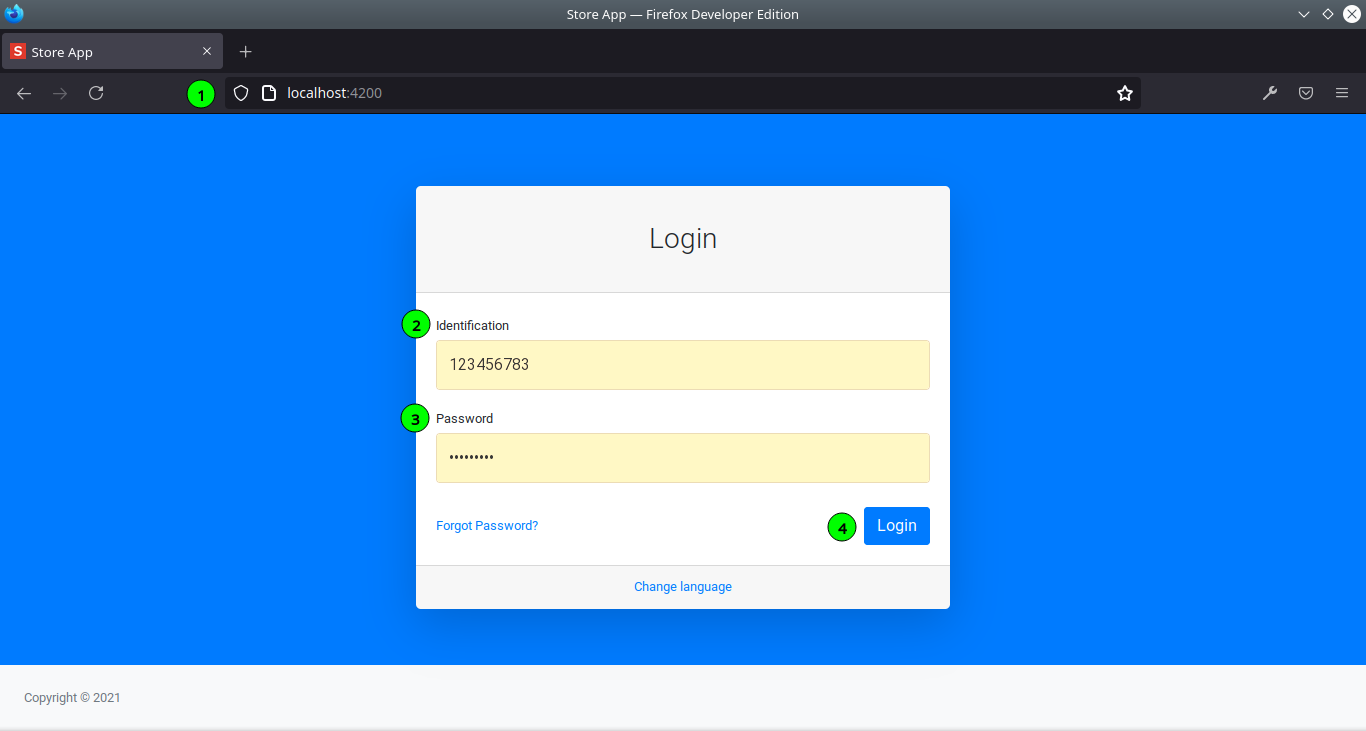
\includegraphics[width=\textwidth]{images/login}
	\caption{login in the application}
	\label{fig:login}
\end{figure}
\end{enumerate}	

\section{Main Page}\label{section:main_page}
This page is showed at access to the system.
\begin{figure}[H]\centering
	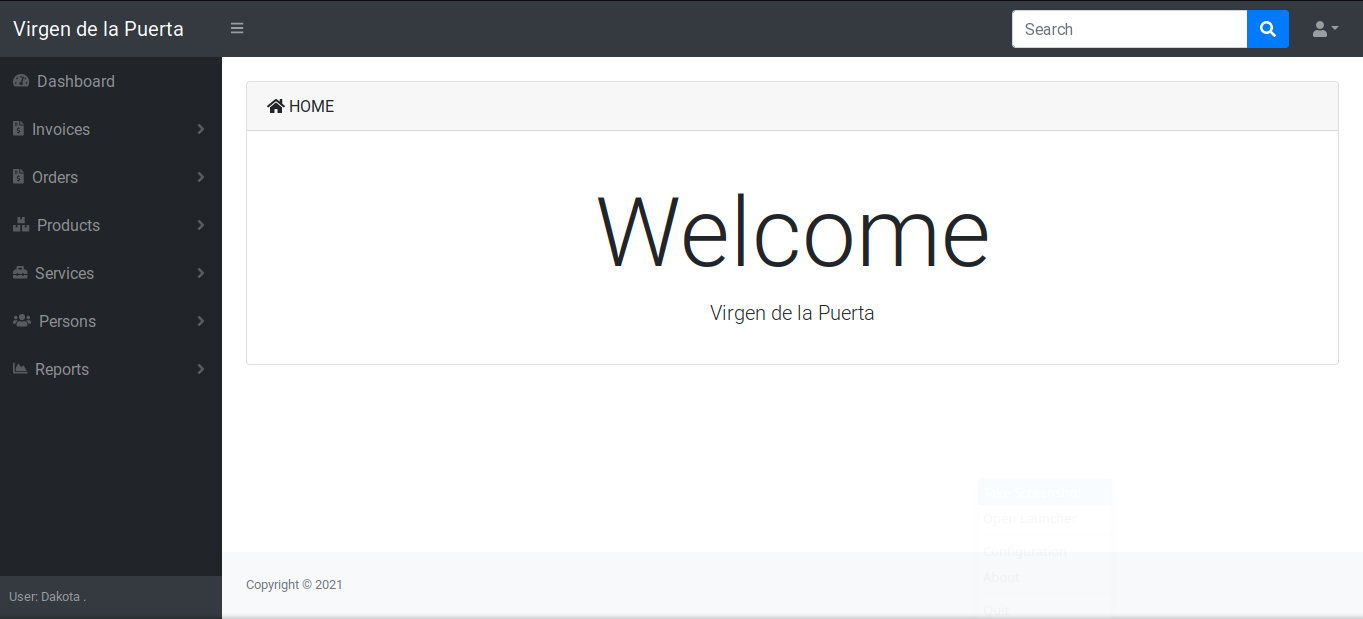
\includegraphics[width=\textwidth]{images/main_page}
	\caption{main page}
	\label{fig:main_page}
\end{figure}

\section{Dashboard}
\subsection{Access to module}
\begin{enumerate}
	\item From the left menu, click in  \menu{Dashboard}
	\item The page will be showed.
	\begin{figure}[H]\centering
		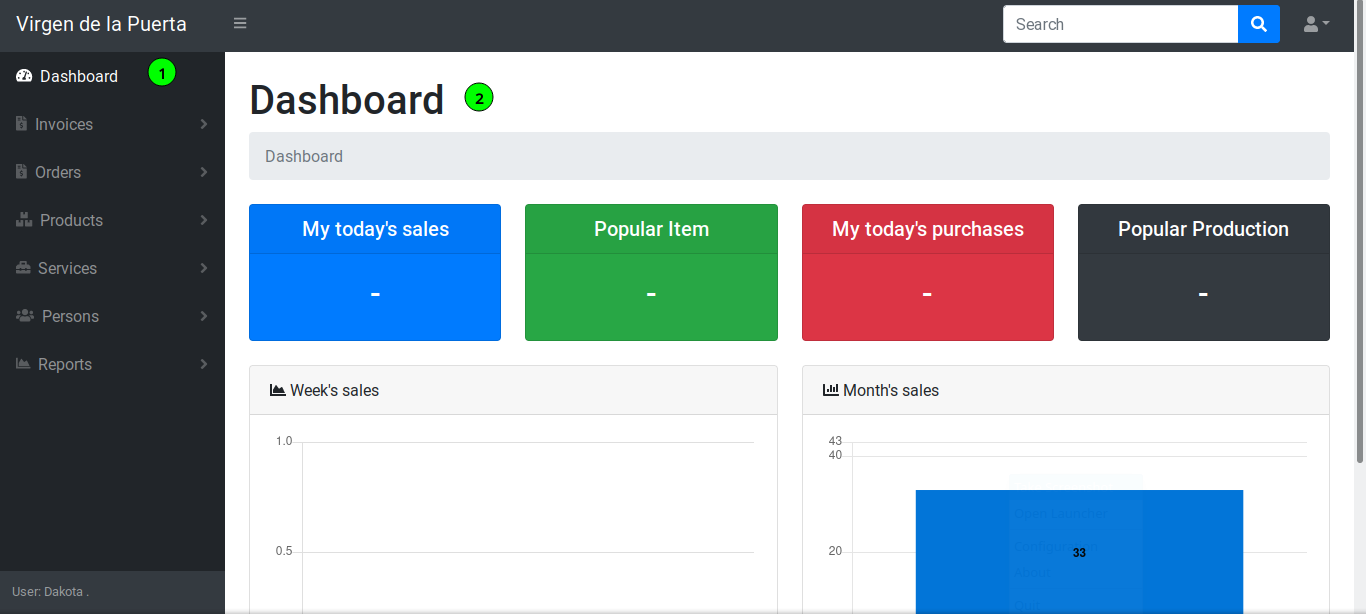
\includegraphics[width=\textwidth]{images/dashboard-access.png}
		\caption{access to module: Dashboard}
		\label{fig:dashboard-access}
	\end{figure}
\end{enumerate}
\subsection{Features}
\begin{enumerate}
	\item \textbf{My todays' sales}: amount of money from sells in the current day.
	\item \textbf{Popular item}: name of item that is the most sell in the current day. 
	\item \textbf{My todays' sales}: amount of money from purchases in the current day.
	\item \textbf{Popular Production}: name of item that is the most produce in the current day. 
		\medskip
	\begin{leftbar}
	 \InConstruction.
	\end{leftbar} 
	\item \textbf{Week's sales}: amount of money from sells in the current week.
	\item \textbf{Month's sales}: amount of money from sells in the current month.
	\begin{figure}[H]\centering
		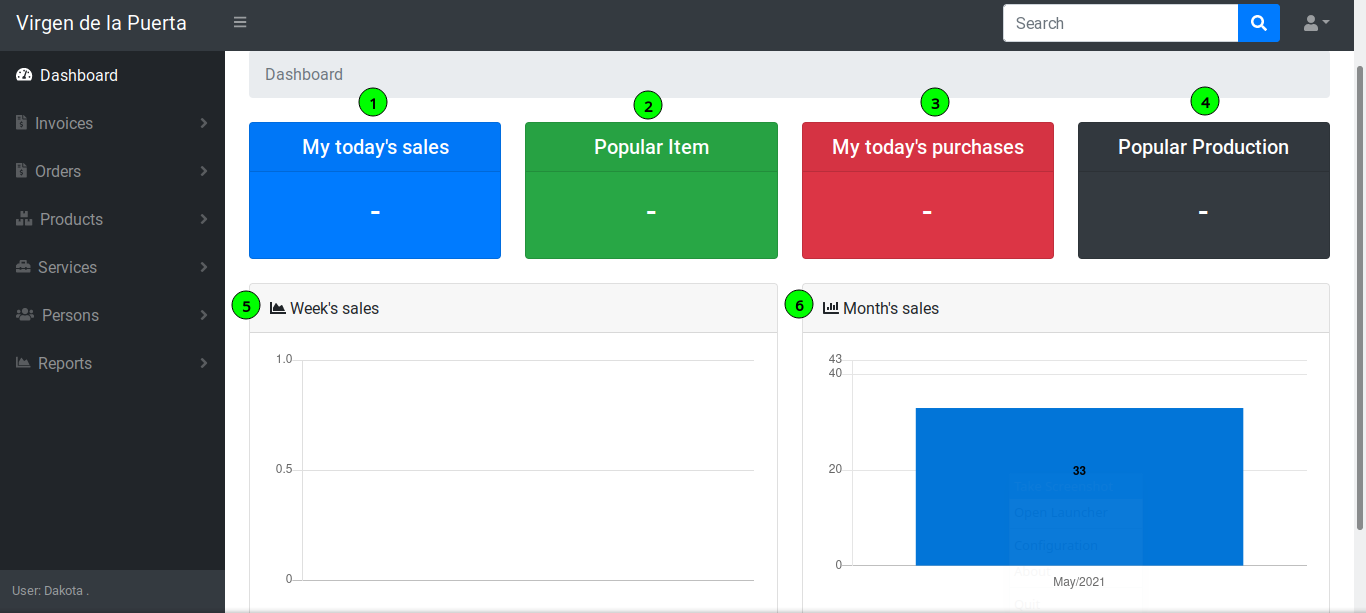
\includegraphics[width=\textwidth]{images/dashboard}
		\caption{dashboard features}
		\label{fig:dashboard}
	\end{figure}
\end{enumerate}
	
\section{Invoices}
\subsection{Invoice List}\label{section:invoice_list}
\subsubsection{Access to module}
\begin{enumerate}
	\item From the left menu, click in  \menu{Invoices}
	\item From the left submenu, click in  \menu{Invoices List}
	\item The page will be showed.
	\medskip
	\begin{leftbar}
		Here there are some action that can be done with the items in the grid such as: \emph{search, made a payment, show and annul} .
	\end{leftbar}
	\begin{figure}[H]\centering
		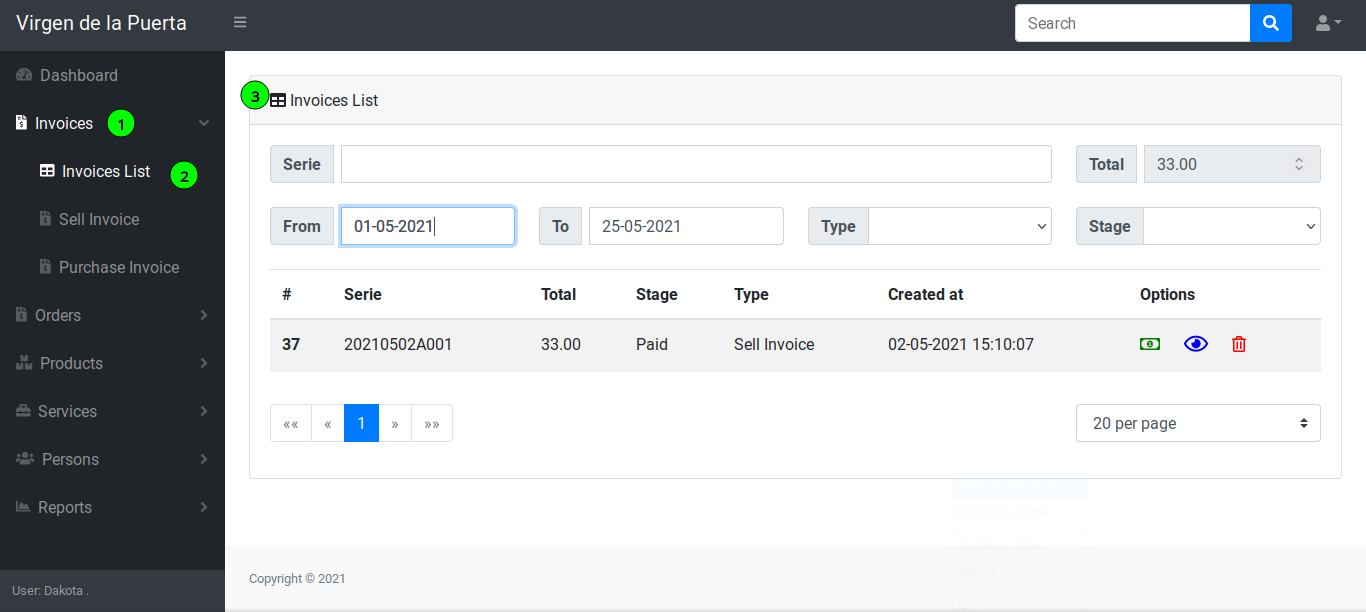
\includegraphics[width=\textwidth]{images/invoice_list-access.png}
		\caption{access to module: Invoice List}
		\label{fig:invoice_list-access}
	\end{figure}
\end{enumerate}

\subsubsection{Search invoice: fields}\label{invoice:invoice_search}
After select or fulfill any field the search will be automatically.
\begin{enumerate}
	\item \textbf{Serie}: invoice serie's number.
	\item \textbf{Total}: this fields is read-only and shows the total amount of all invoice listed.
	\item \textbf{From}: initial date in search range.
	\item \textbf{To}: final date in search range.
	\item \textbf{Type}: it is the type of invoice and it can selected one option or in blank, which means will search for all.
		\medskip
		\begin{leftbar}
			Options: \emph{sell or purchase} .
		\end{leftbar}
	\item \textbf{Stage}: It is the status of the invoice and it can selected one option or in blank, which means will search for both.
		\medskip
		\begin{leftbar}
			Options: \emph{paid, annulled, draft, by installment and no paid} .
		\end{leftbar}
	
	\begin{figure}[H]\centering
		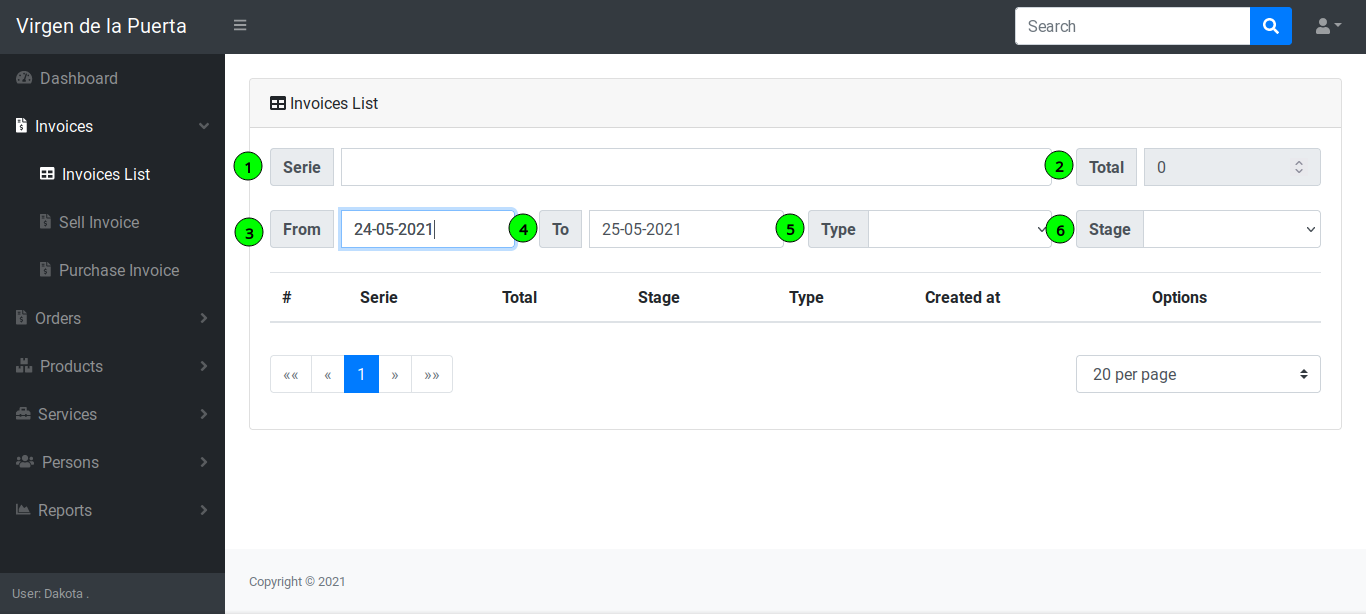
\includegraphics[width=\textwidth]{images/invoice_list-search-fields.png}
		\caption{search invoice: fields}
		\label{fig:invoice_list-search-fields}
	\end{figure}
\end{enumerate}

\subsubsection{Made payment}
\begin{enumerate}
	\item Find the invoice to pay.
	\item Click in \faIcon{money-bill-alt}.
	\medskip
	\begin{leftbar}
		A modal will be open, go to (Section~\ref{section:made_payment}) to continue this workflow.
	\end{leftbar}
	\begin{figure}[H]\centering
		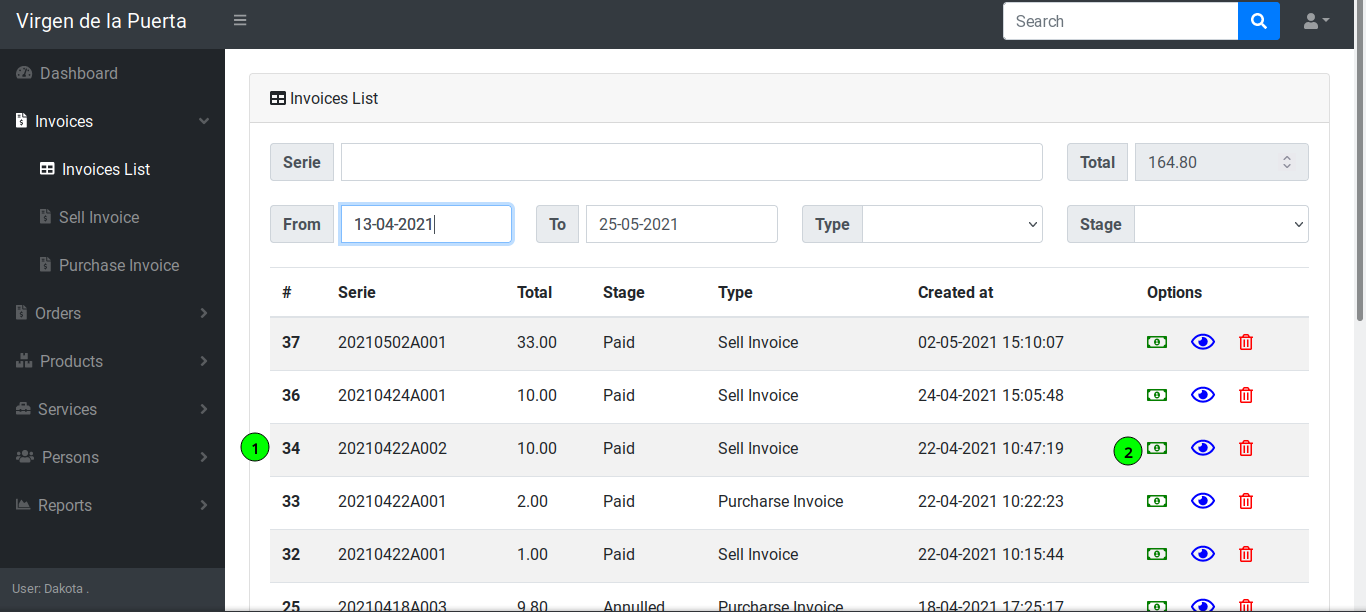
\includegraphics[width=\textwidth]{images/invoice_list-made-payment.png}
		\caption{Made Payment}
		\label{fig:invoice_list-made-payment}
	\end{figure}
\end{enumerate}

\subsubsection{Show invoice's information}
\begin{enumerate}
	\item Find the invoice to show its information.
	\item Click in \faIcon{eye}.
	\begin{figure}[H]\centering
		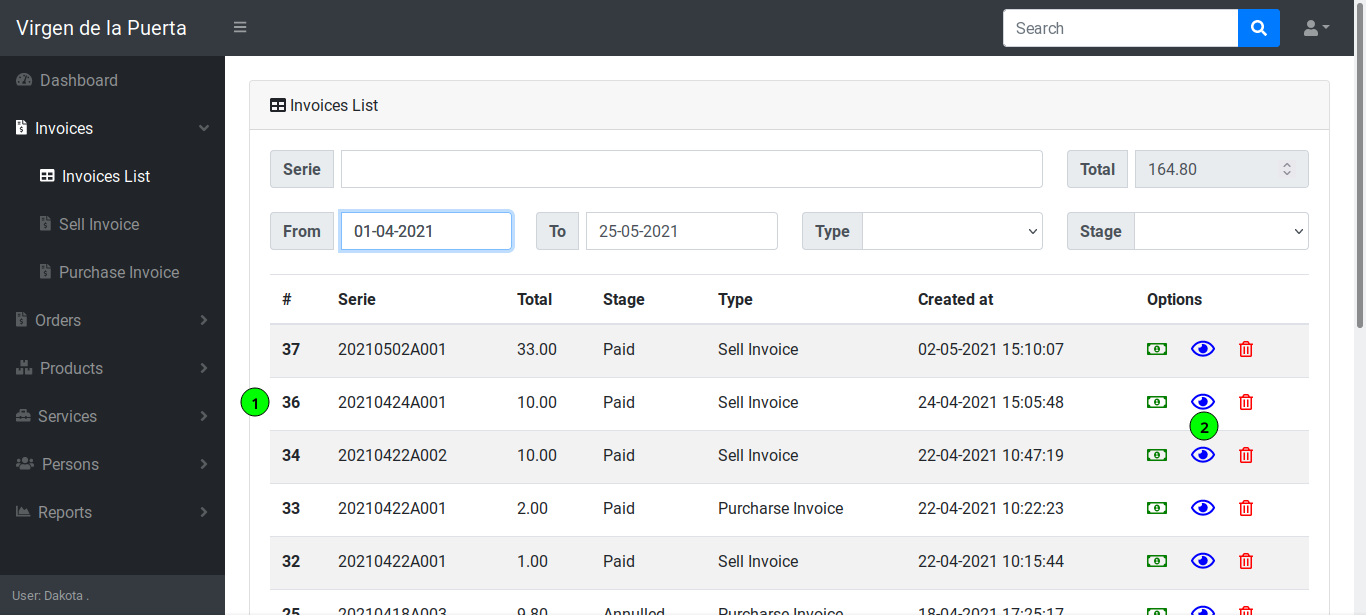
\includegraphics[width=\textwidth]{images/invoice_list-show.png}
		\caption{show invoice's information}
		\label{fig:invoice_list-show}
	\end{figure}
	\item The information is showed.
	\item Click in \keys{print} to print the invoice; otherwise, Click in \keys{close} to close the modal.
	\begin{figure}[H]\centering
		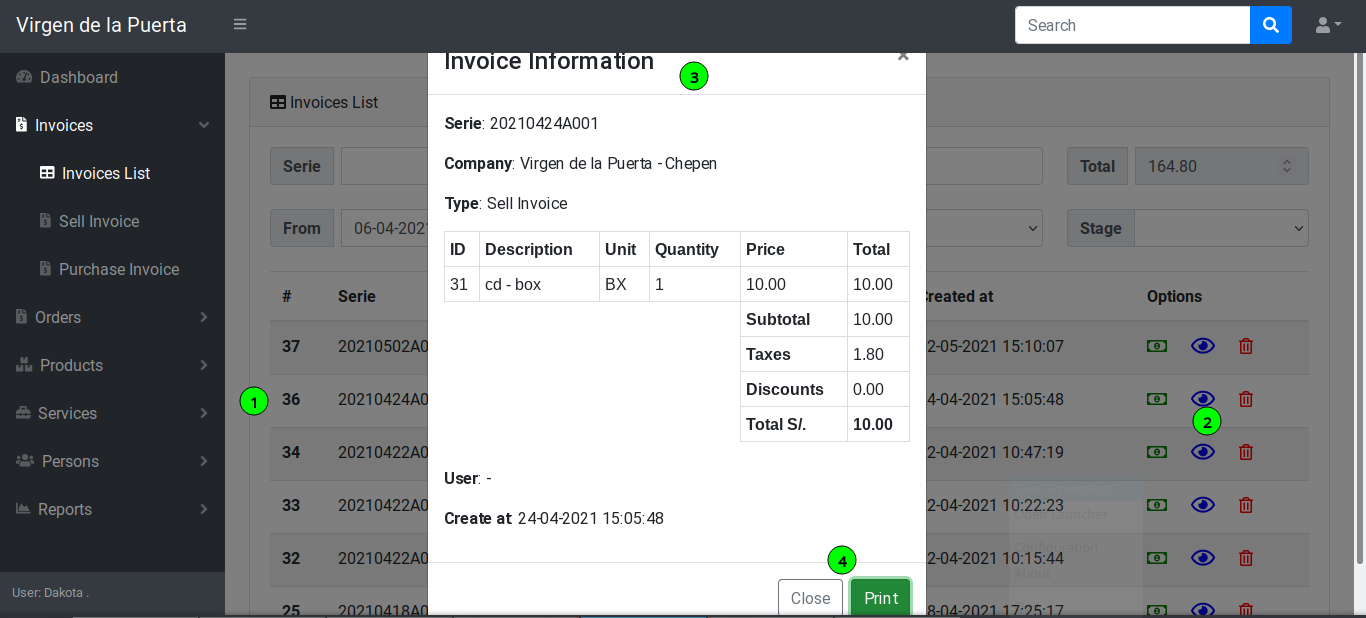
\includegraphics[width=\textwidth]{images/invoice_list-show-modal.png}
			\caption{show invoice's information: modal}
		\label{fig:invoice_list-show-modal}
	\end{figure}
\end{enumerate}

\subsubsection{Annul invoice}
\begin{enumerate}
	\item Find the invoice to annul.
	\item Click in \faIcon{trash}.
	\begin{figure}[H]\centering
		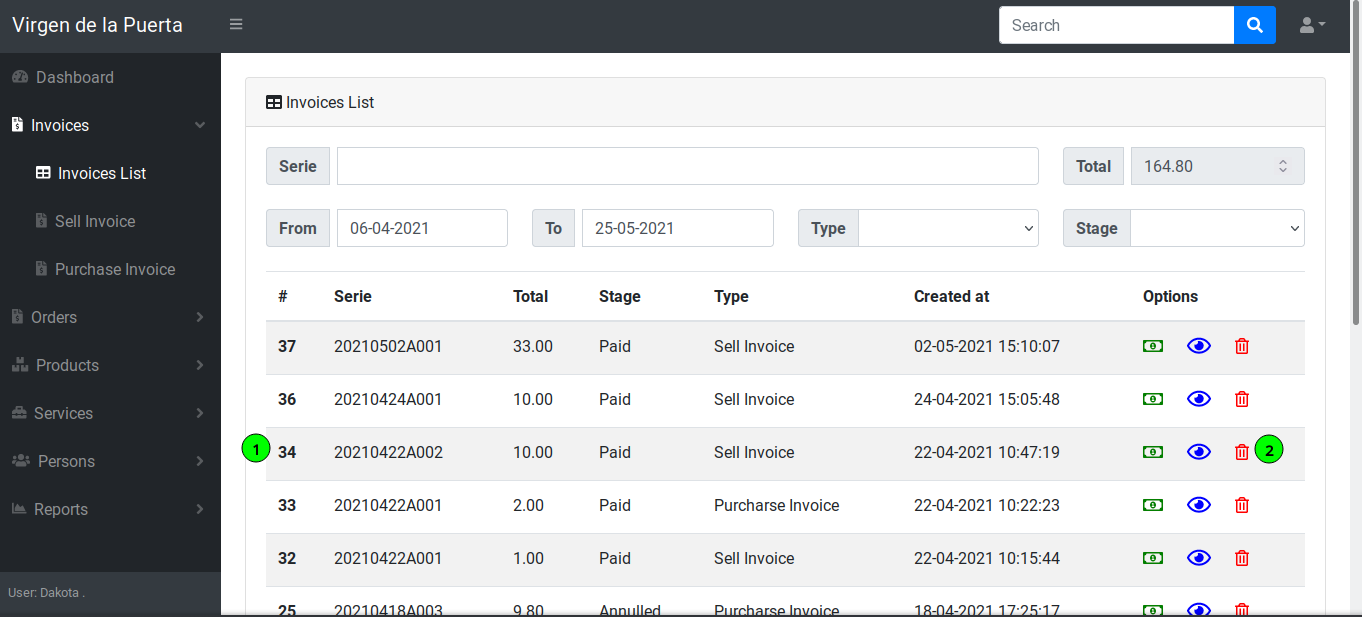
\includegraphics[width=\textwidth]{images/invoice_list-annul.png}
		\caption{annul invoice}
		\label{fig:invoice_list-annul}
	\end{figure}
	\item Click in \keys{yes} to confirm the annul; otherwise, Click in \keys{cancel} to abort the process.
	\begin{figure}[H]\centering
		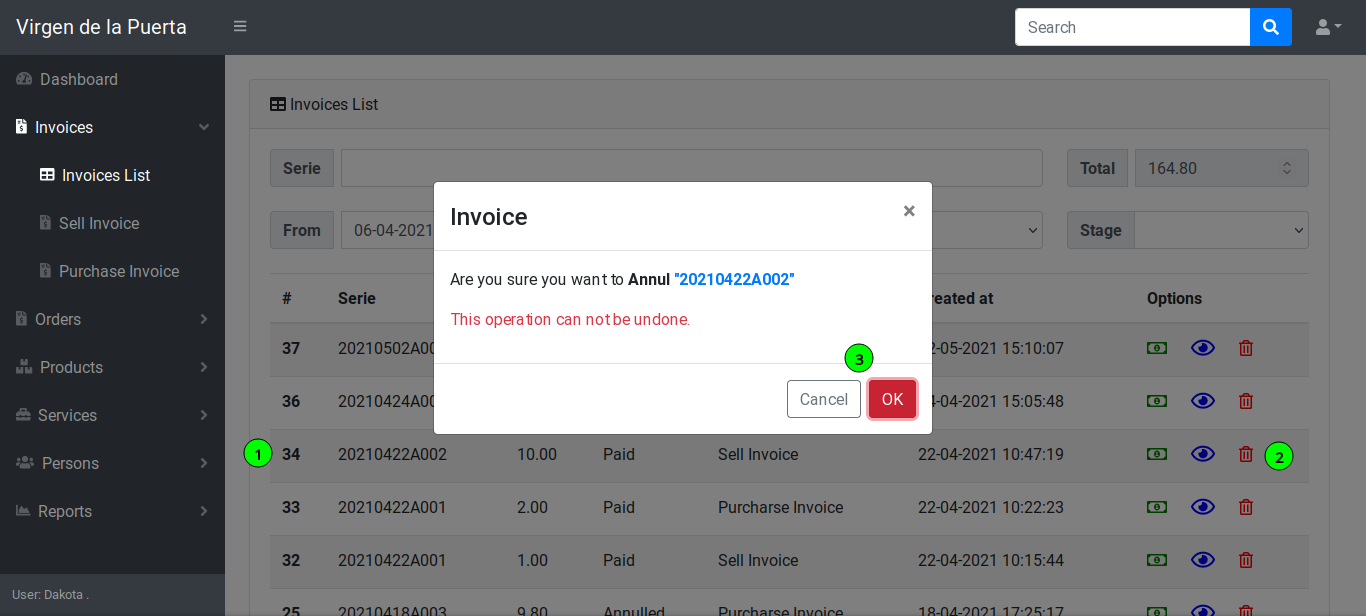
\includegraphics[width=\textwidth]{images/invoice_list-annul-modal.png}
		\caption{annul invoice: modal}
		\label{fig:invoice_list-annul-modal}
	\end{figure}
\end{enumerate}

\subsection{To Sell}\label{section:to_sell}
\subsubsection{Access to module: Sell}
\begin{enumerate}
	\item From the left menu, click in  \menu{Invoices}
	\item From the left submenu, click in  \menu{Sell invoice}
	\item The page will be showed.
	\begin{figure}[H]\centering
		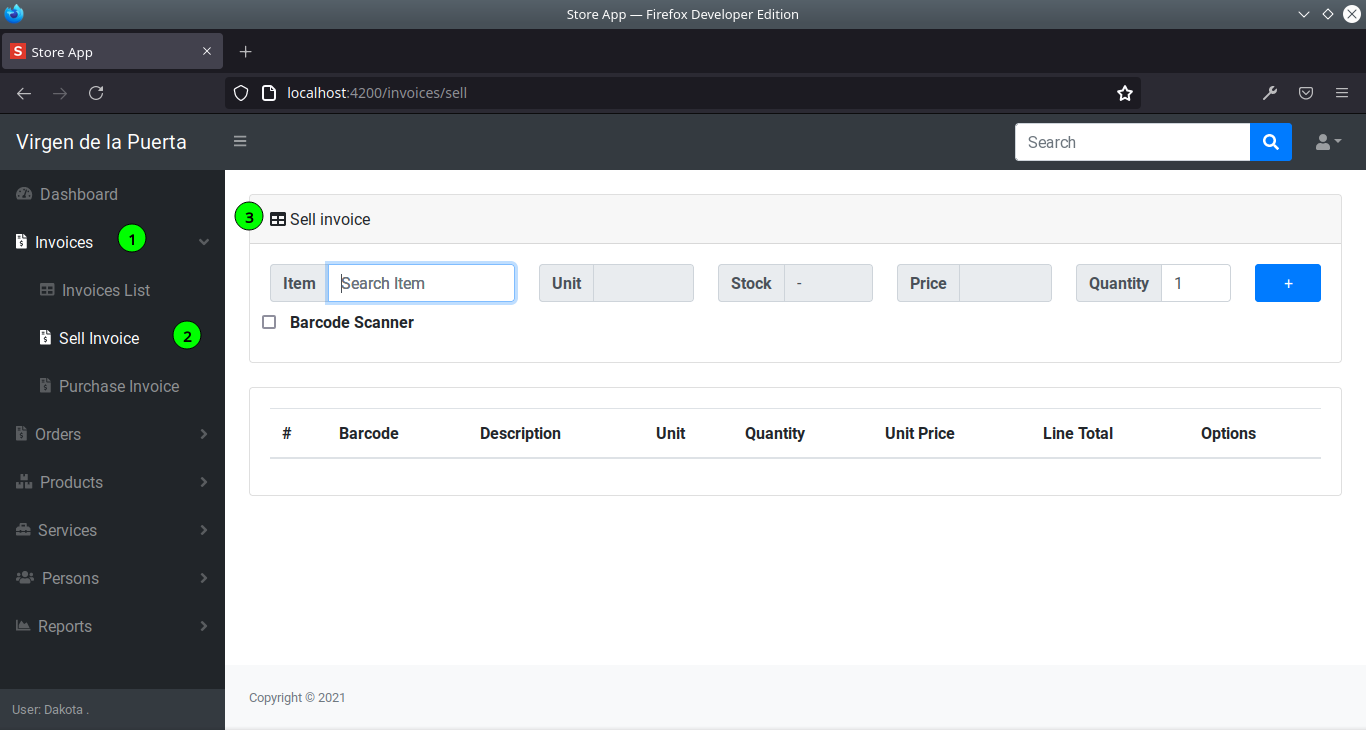
\includegraphics[width=\textwidth]{images/invoice_sell-access}
		\caption{access to module: Sell}
		\label{fig:invoice_sell-access}
	\end{figure}
\end{enumerate}

\subsubsection{Add an item}
\begin{enumerate}
	\item Search item, \emph{write the first letters of item name and it will be auto-completed.}
	\medskip
	\begin{leftbar}
		It will show item's information such as \emph{ unit, stock and price}
	\end{leftbar}
	\item Write quantity.
	\item Click in \keys{\texttt{+}}
	\medskip
	\begin{leftbar}
		The item will be showed in the grill,  \emph{with some additional information}
	\end{leftbar}
	\begin{figure}[H]\centering
		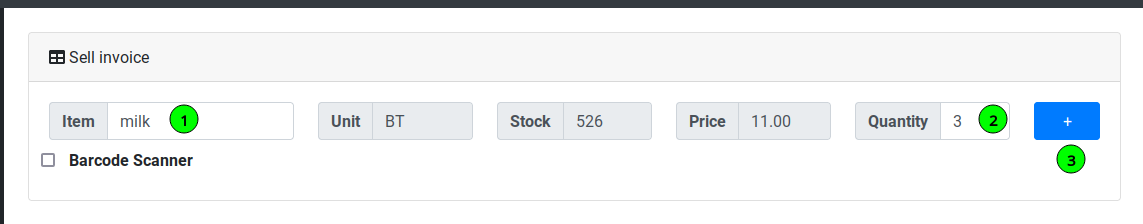
\includegraphics[width=\textwidth]{images/invoice_sell-item}
		\caption{add an item}\label{fig:invoice_sell-item}
	\end{figure}
\end{enumerate}

\subsubsection{Show item in grill}
\begin{enumerate}
	\item in that section, the item is showed in the grill,  \emph{with some additional fields}
	\medskip
	\begin{leftbar}
		It will show item's information such as \emph{ index, barcode, unit, quantity, unit price, line total and delete button}
	\end{leftbar}
	\item in that section, information about \emph{subtotal, taxes, discount and total} is showed
	\medskip
	\begin{leftbar}
	To make a discount check its section.
	\end{leftbar}
	\begin{figure}[H]\centering
		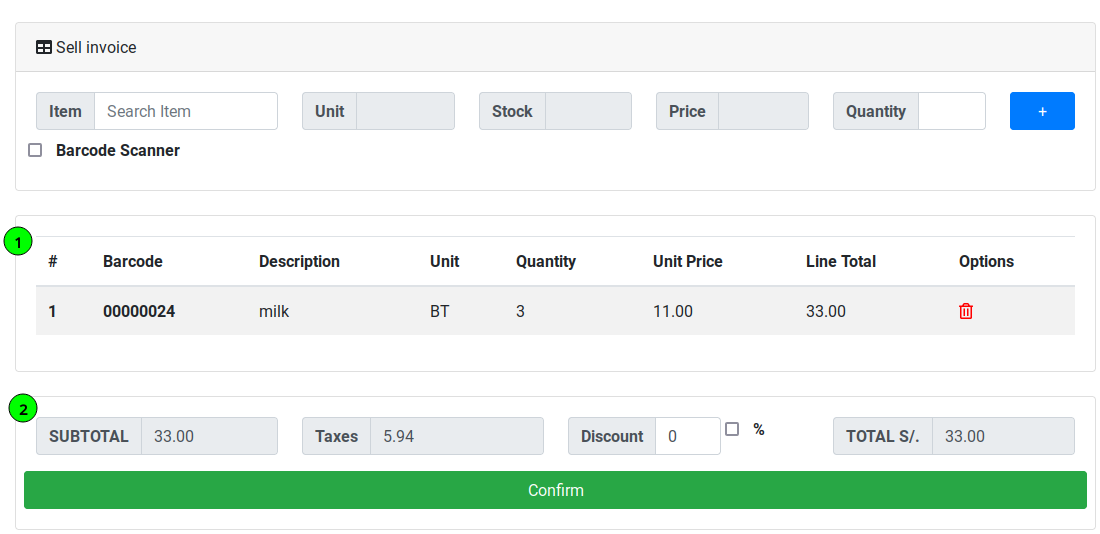
\includegraphics[width=\textwidth]{images/invoice_sell-grill}
		\caption{show item in grill}\label{fig:invoice_sell-grill}
	\end{figure}
\end{enumerate}

\subsubsection{Confirm sell}
\begin{enumerate}
	\item Click in \keys{Confirm} 
	\begin{figure}[H]\centering
		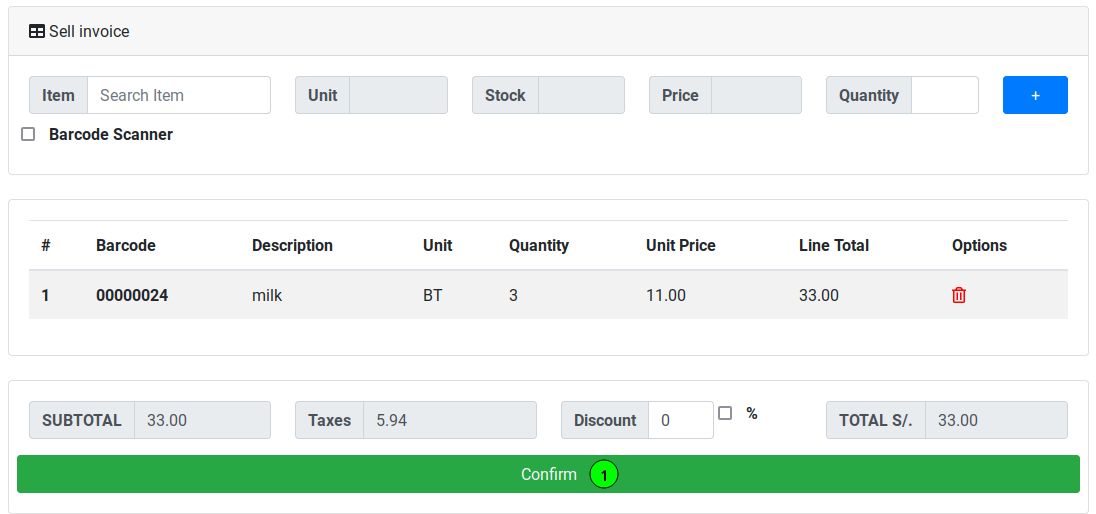
\includegraphics[width=\textwidth]{images/invoice_sell-confirm}
		\caption{confirm sell}\label{fig:invoice_sell-confirm}
	\end{figure}
	\item Go to (Section~\ref{section:invoice_additional_information}) to continue the workflow.
\end{enumerate}

%\subsubsection{Show sell invoice}

\subsection{To Purchase}\label{section:to_purchase}
\subsubsection{Access to module: Purchase}
\begin{enumerate}
	\item From the left menu, click in  \menu{Invoices}
	\item From the left submenu, click in  \menu{Purchase invoice}
	\item The page will be showed.
	\begin{figure}[H]\centering
		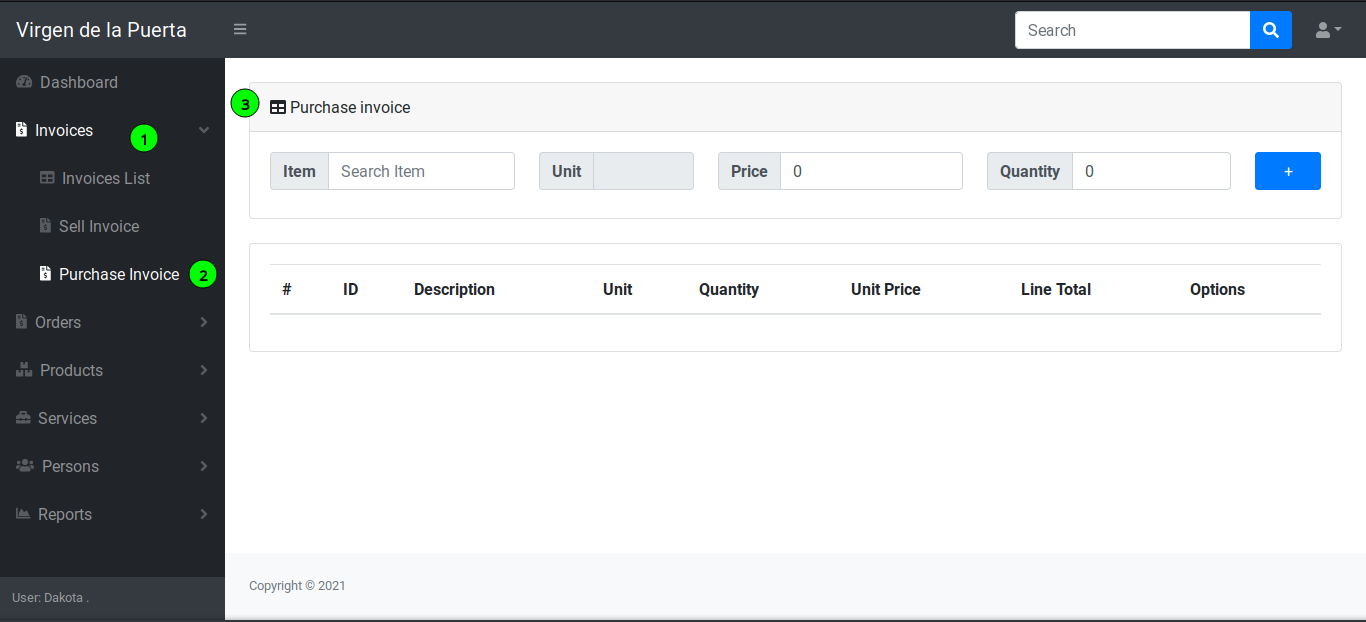
\includegraphics[width=\textwidth]{images/invoice_purchase-access.png}
		\caption{access to module: Purchase}
		\label{fig:invoice_purchase-access}
	\end{figure}
\end{enumerate}

\subsubsection{Add an item}
\begin{enumerate}
	\item Search item, \emph{write the first letters of item name and it will be auto-completed.}
	
	\medskip
	\begin{leftbar}
		It will show item's information such as \emph{ unit, stock and price}
	\end{leftbar}
	\item Write purchase's price.
	\item Write quantity.
	\item Click in \keys{\texttt{+}}

	\medskip
	\begin{leftbar}
		The item will be showed in the grill,  \emph{with some additional information.}
	\end{leftbar}
	\begin{figure}[H]\centering
		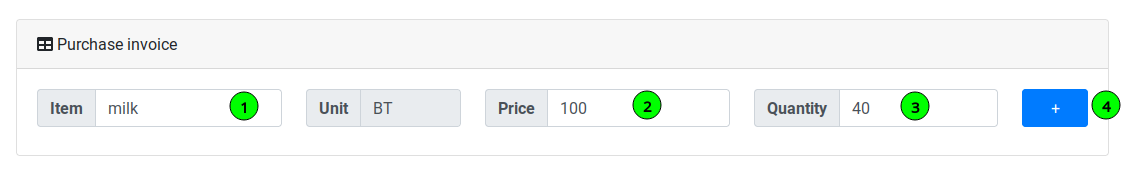
\includegraphics[width=\textwidth]{images/invoice_purchase-item.png}
		\caption{add an item}\label{fig:invoice_purchase-item}
	\end{figure}
\end{enumerate}

\subsubsection{Show item in grill}
\begin{enumerate}
	\item In that section, the item is showed in the grill,  \emph{with some additional fields}
	\medskip
	\begin{leftbar}
		It will show item's information such as \emph{ index, barcode, description, unit, quantity, unit price, line total and delete button.}
	\end{leftbar}
	\item In that section, information about \emph{subtotal, taxes, discount and total} is showed.
	\medskip
	\begin{leftbar}
		To make a discount check its section.
	\end{leftbar}
	\begin{figure}[H]\centering
		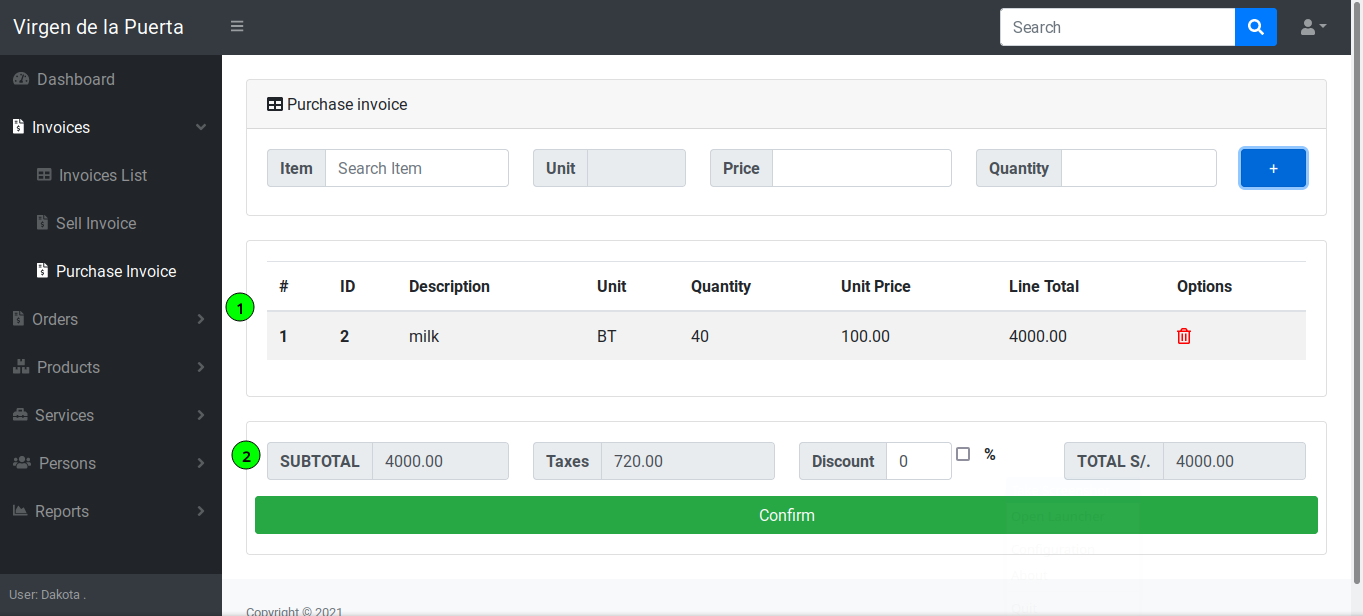
\includegraphics[width=\textwidth]{images/invoice_purchase-grill.png}
		\caption{show item in grill}\label{fig:invoice_purchase-grill}
	\end{figure}
\end{enumerate}

\subsubsection{Confirm purchase}
\begin{enumerate}
	\item Click in \keys{Confirm} 
	\begin{figure}[H]\centering
		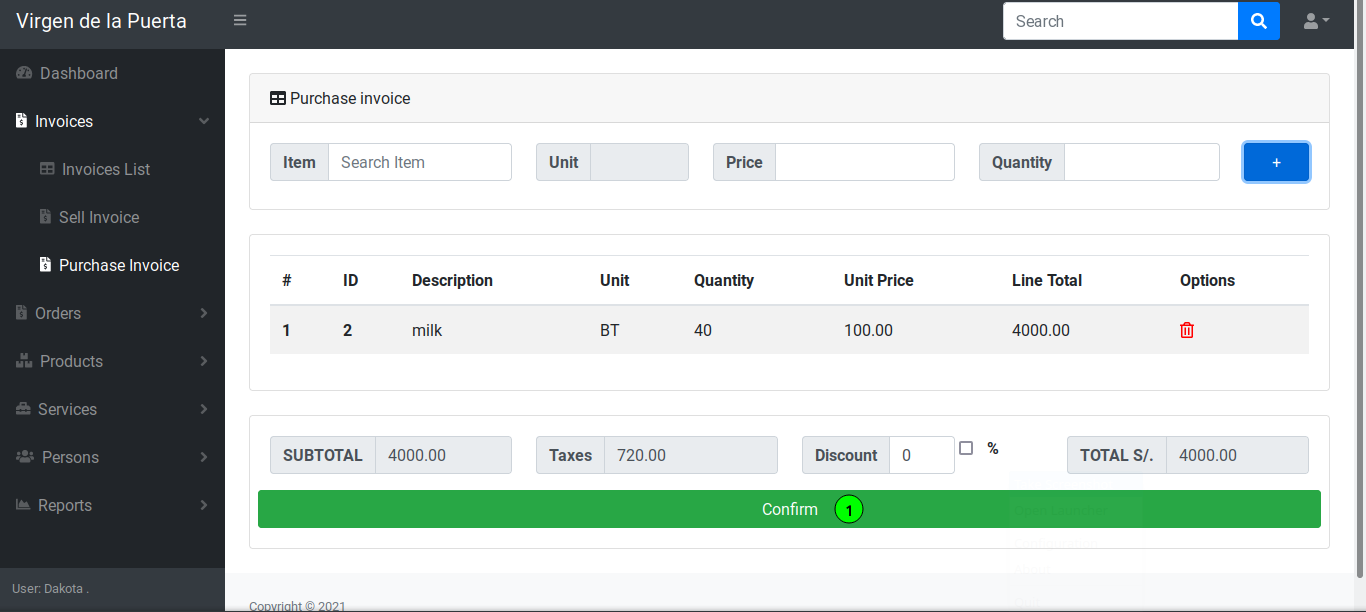
\includegraphics[width=\textwidth]{images/invoice_purchase-confirm.png}
		\caption{confirm purchase}
		\label{fig:invoice_purchase-confirm}
	\end{figure}
	\item Go to (Section~\ref{section:invoice_additional_information}) to continue the workflow.
\end{enumerate}

\subsection{Invoice additional information}\label{section:invoice_additional_information}
This workflow depends on the option that is selected for \emph{payment type} which are the next ones:
\begin{itemize}
	\item Credit
	\item Debit
	\item Cash
	\item Store Credit
\end{itemize}
\subsubsection{Payment type: Credit or Debit}
\begin{enumerate}
	\item Select payment type \textbf{CREDIT} or \textbf{DEBIT}	.
	\item Select a client, \emph{write its name or identification number}.
	\medskip
	\begin{leftbar}
		\textbf{OPTIONAL FIELD}
	\end{leftbar}
	\item Click in \keys{Finish} 	
	\medskip
	\begin{leftbar}
		The process will be finished and the user will redirected to \textbf{Invoice List} page in (Section~\ref{section:invoice_list}).
	\end{leftbar}
	\begin{figure}[H]\centering
		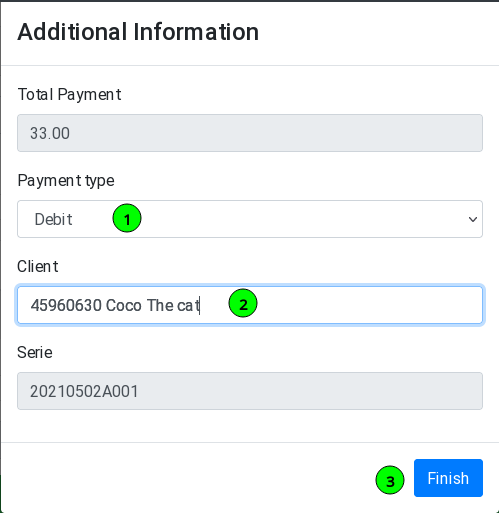
\includegraphics[width=\textwidth]{images/sellinvoice-5}
		\caption{Add additional information: Credit or Debit}\label{fig:sellinvoice-5}
	\end{figure}
\end{enumerate}

\subsubsection{Payment type: Cash}
\begin{enumerate}
	\item Select payment type \textbf{CASH}.
	\item Select a client, \emph{write its name or identification number}.
	\medskip
	\begin{leftbar}
		\textbf{OPTIONAL FIELD}
	\end{leftbar}
	\item Click in \keys{Next} 	
	\medskip
	\begin{figure}[H]\centering
		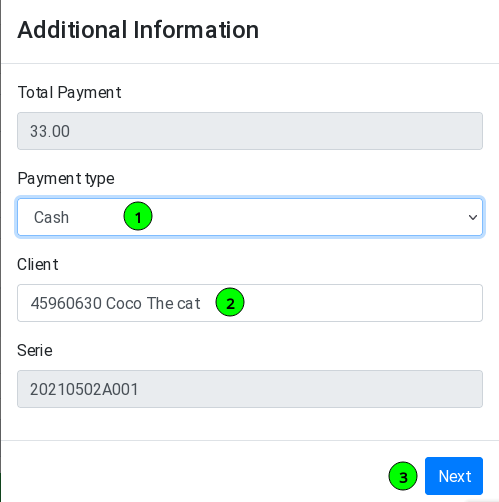
\includegraphics[width=\textwidth]{images/sellinvoice-6}
		\caption{add additional information: Cash}\label{fig:sellinvoice-6}
	\end{figure}
	\item It will be redirected to make the payment in  (Section~\ref{section:made_payment}) and continue the workflow.
\end{enumerate}
\section{Products}
\subsection{Product List}\label{section:product_list}
\subsubsection{Access to module}
\begin{enumerate}
	\item From the left menu, click in  \menu{Products}
	\item From the left submenu, click in  \menu{Products List}
	\item The page will be showed.
	\medskip
	\begin{leftbar}
		Here there are some action that can be done with the items in the grid such as: \emph{search, edit, delete and print} .
	\end{leftbar}
	\begin{figure}[H]\centering
		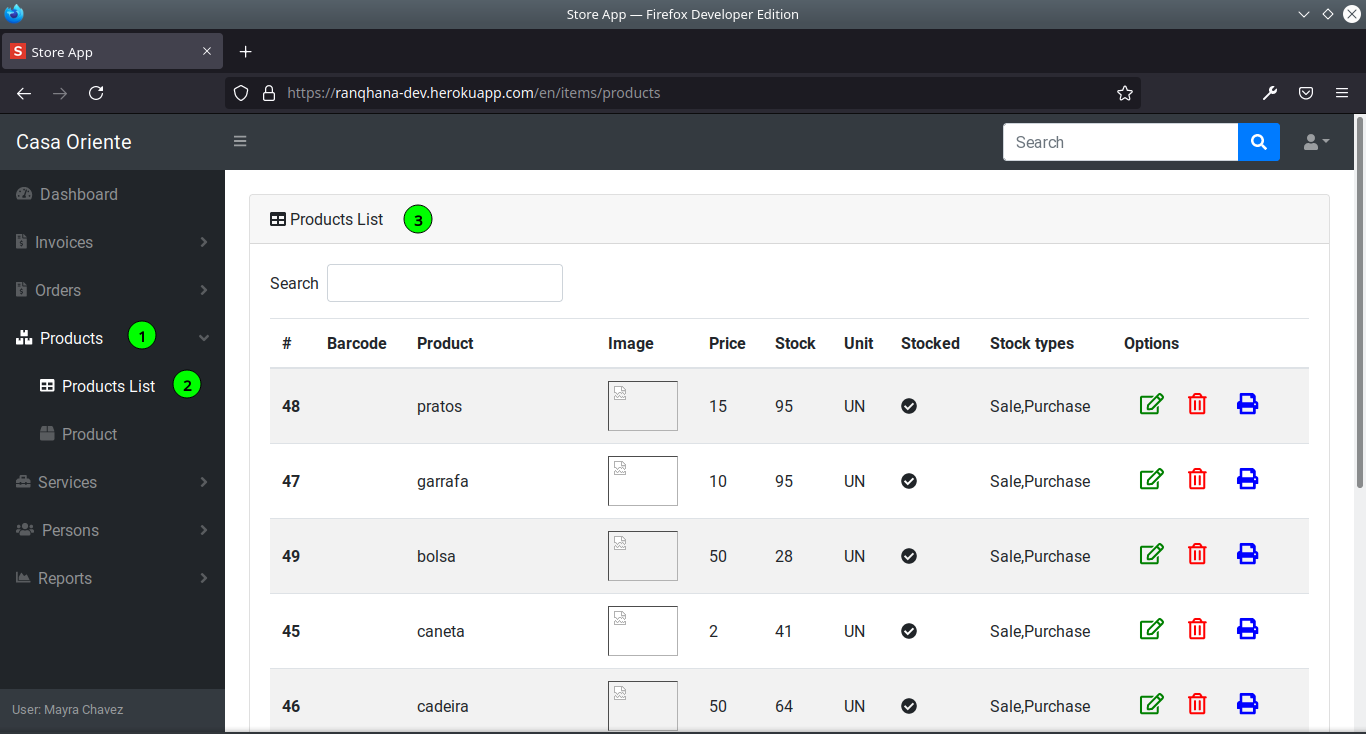
\includegraphics[width=\textwidth]{images/produc_list-access.png}
		\caption{access to module: Product List}
		\label{fig:produc_list-access.png}
	\end{figure}
\end{enumerate}

\subsubsection{Search product}\label{section:product_search}
\begin{enumerate}
	\item Write product name or part of that and it will be searched automatically.
	\begin{figure}[H]\centering
		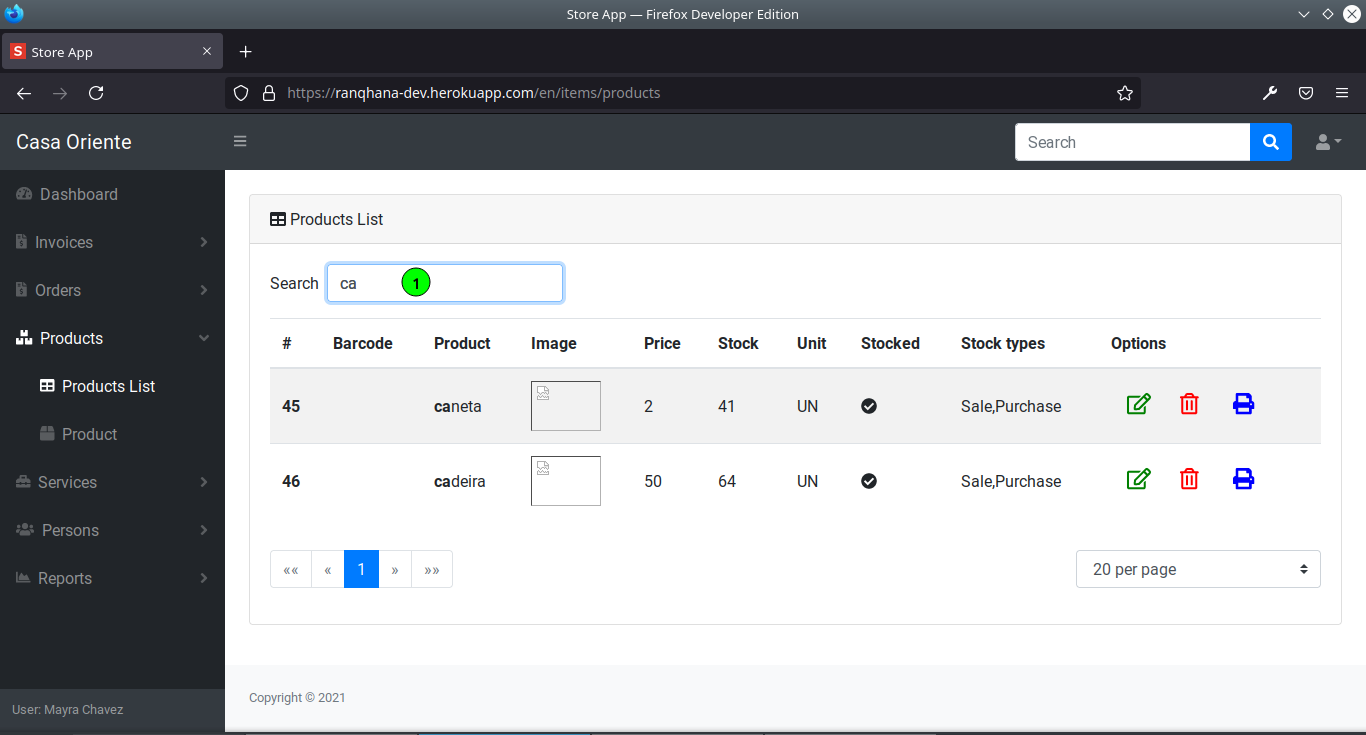
\includegraphics[width=\textwidth]{images/produc_list-search.png}
		\caption{search product}
		\label{fig:produc_list-search.png}
	\end{figure}
\end{enumerate}

\subsubsection{Delete product}
\begin{enumerate}
	\item Find the product to delete.
	\item Click in \faIcon{trash}.
		\begin{figure}[H]\centering
			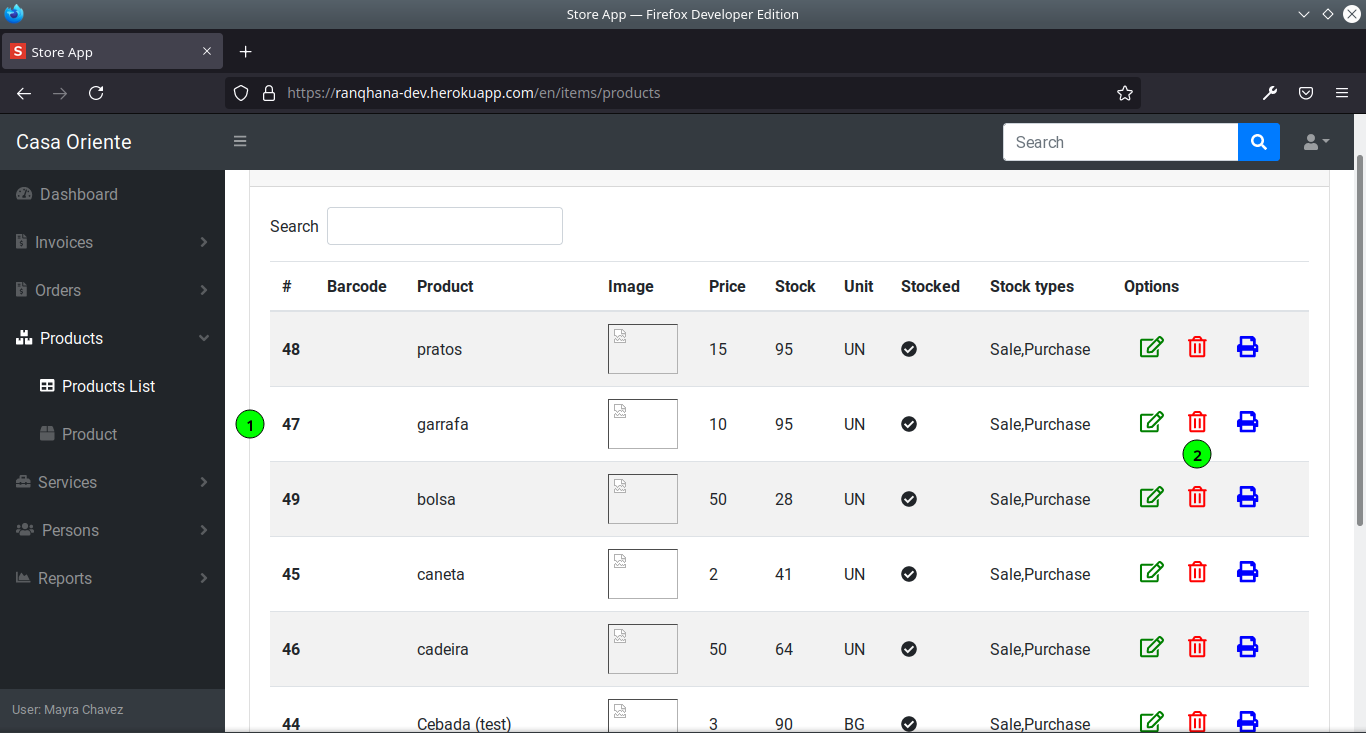
\includegraphics[width=\textwidth]{images/produc_list-delete.png}
			\caption{delete product}
			\label{fig:produc_list-delete.png}
		\end{figure}
	\item Click in \keys{yes} to confirm the delete; otherwise, Click in \keys{cancel} to abort the process.
	\begin{figure}[H]\centering
		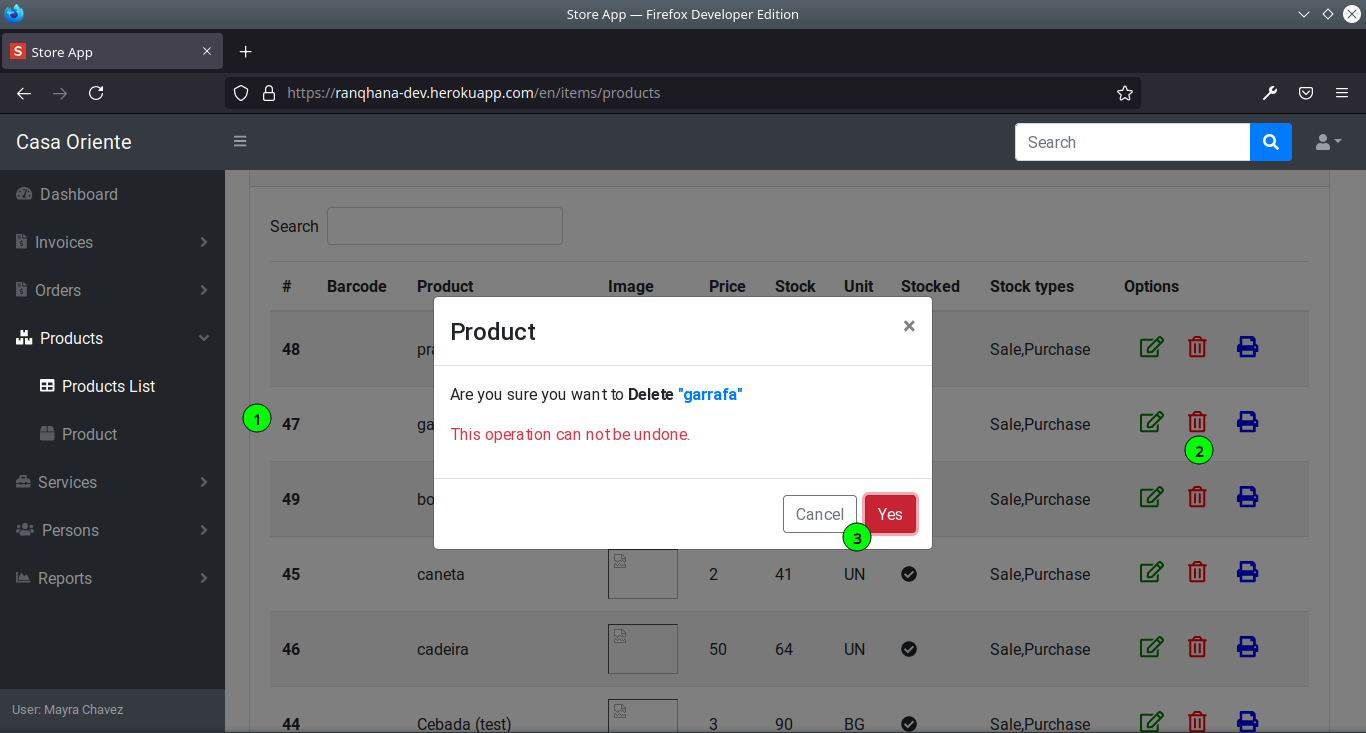
\includegraphics[width=\textwidth]{images/produc_list-delete-modal.png}
		\caption{delete product: modal}
		\label{fig:produc_list-delete-modal.png}
	\end{figure}
\end{enumerate}

\subsubsection{Update/Edit product}
\begin{enumerate}
	\item Find the product to edit.
	\item Click in \faIcon{edit}.
	\medskip
	\begin{leftbar}
	 At that moment, it will be redirected to \textbf{Product Form} page in (Section~\ref{section:product_list}).
	\end{leftbar}
	\begin{figure}[H]\centering
		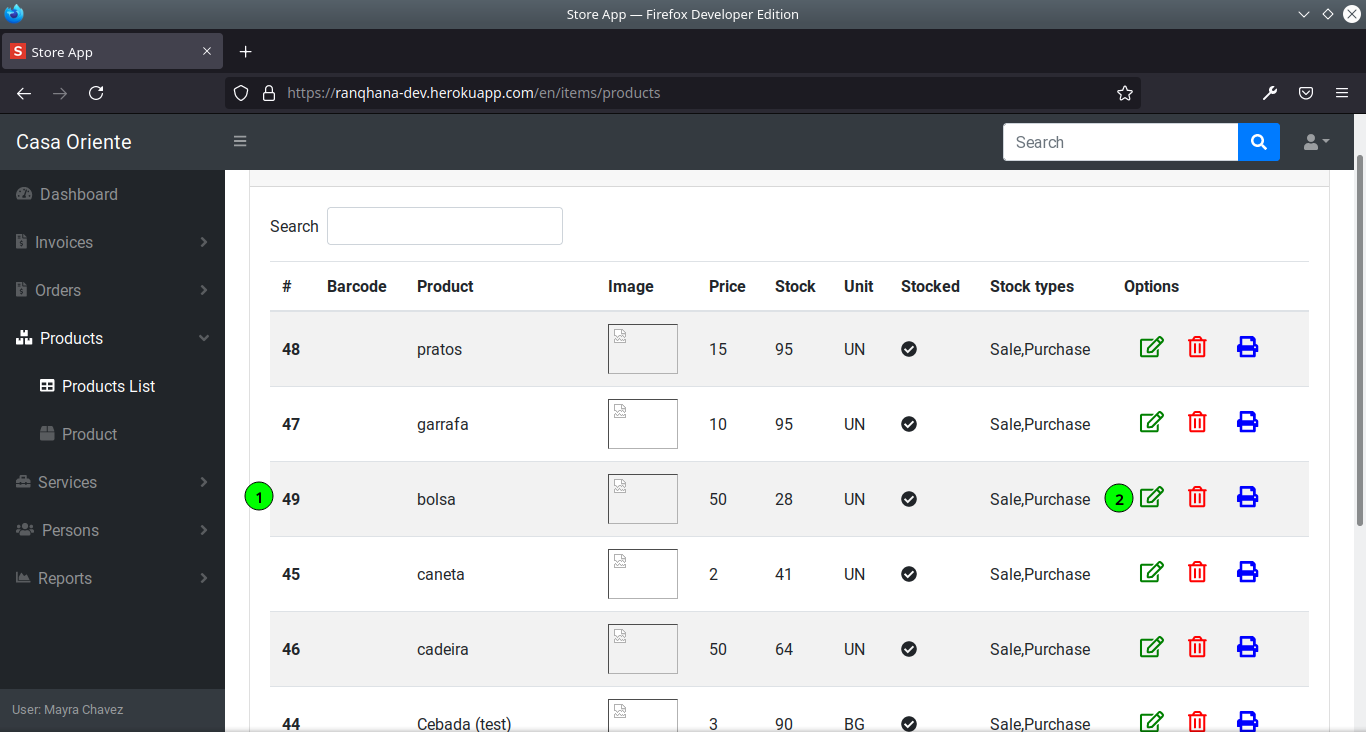
\includegraphics[width=\textwidth]{images/produc_list-update.png}
		\caption{update/edit product}
		\label{fig:produc_list-update.png}.
	\end{figure}
\end{enumerate}

\subsubsection{Print product}
\begin{enumerate}
	\item \InConstruction{}
\end{enumerate}

\subsection{Product form}\label{section:product_form}
\subsubsection{Access to module}
\begin{enumerate}
	\item From the left menu, click in  \menu{Products}
	\item From the left submenu, click in  \menu{Product}
	\item The page will be showed.
	\medskip
	\begin{leftbar}
		Here 2 actions can be performed \emph{create and update} .
	\end{leftbar}
	\begin{figure}[H]\centering
		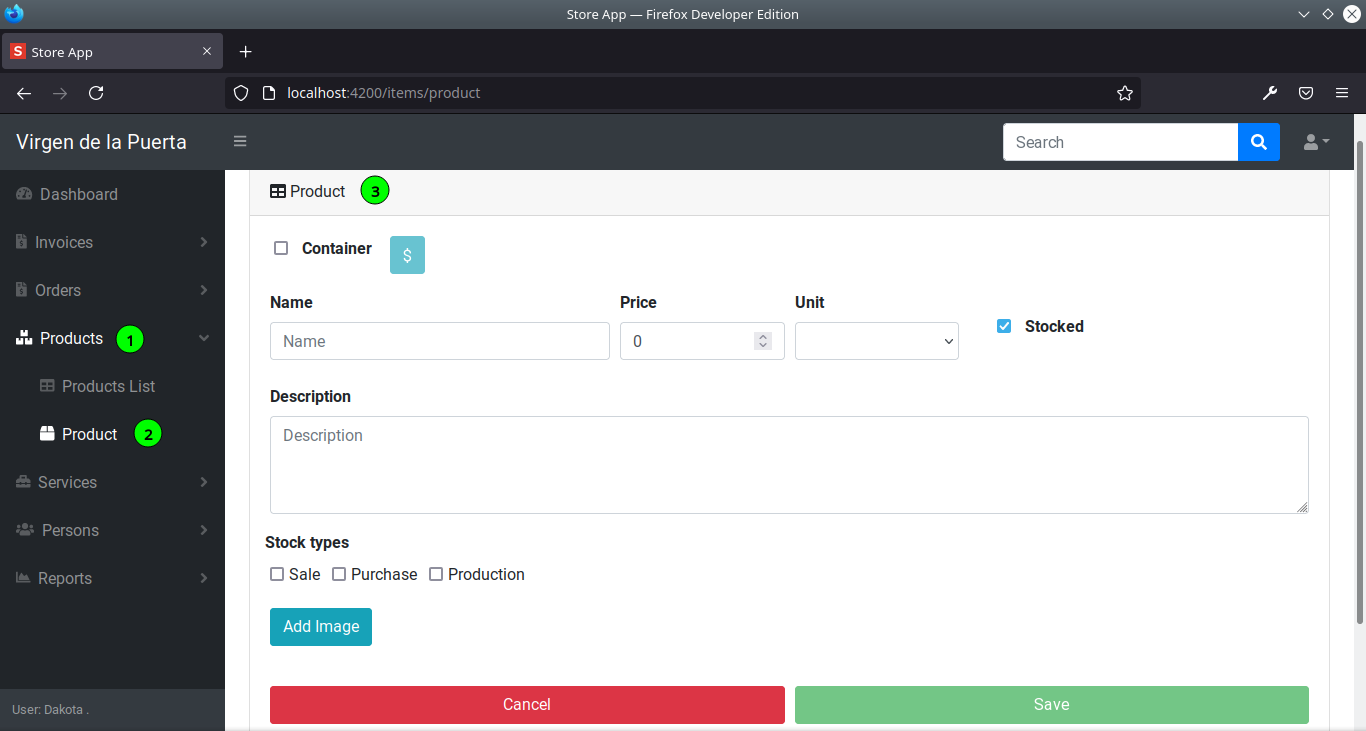
\includegraphics[width=\textwidth]{images/product_form-access.png}
		\caption{access to module: Product}
		\label{fig:product_form-access.png}
	\end{figure}
\end{enumerate}

\subsubsection{Product's field}
\begin{enumerate}
	\item \textbf{Container}: it must be unchecked which means that a product will be created.	
	\item \textbf{Historic pricing}: show sell and purchase's price through time. If its only activate when a product is updated. See (Section~\ref{section:historic_pricing}).
	\item \textbf{Name}: product's name.
	\item \textbf{Price}: product's price.
		\medskip
		\begin{leftbar}
			\textbf{OPTIONAL FIELD}, can be fulfill later.
		\end{leftbar}
	\item \textbf{Unit}: it can be chosen between some options as: \emph{box, bottle, kilogram and so on}
	\item \textbf{Stocked}: check if the product will have stock; otherwise, uncheck it.
	\item \textbf{Description}: product's description.
		\medskip
		\begin{leftbar}
			\textbf{OPTIONAL FIELD}
		\end{leftbar}
	\item \textbf{Stock types}: there are 3 types and they can be selected more than one.
		\begin{enumerate}
			\item \textbf{Sale}: if the product is going to be only sell, but not buy itself.
			\item \textbf{Purchase}: if the product is only bought but not sell.
			\item \textbf{Production}:  \InConstruction{}
		\end{enumerate}
	\item \textbf{Add image}: add product's image. See in (Section~\ref{section:add_image}).
		\medskip
		\begin{leftbar}
			\textbf{OPTIONAL FIELD}.
		\end{leftbar}
	\item Click in \keys{save} to confirm the process; otherwise, Click in \keys{cancel} to abort it.
		\medskip
		\begin{leftbar}
			The process will be finished and the user will redirected to \textbf{Product List} page in (Section~\ref{section:product_list}).
		\end{leftbar}
	\begin{figure}[H]\centering
		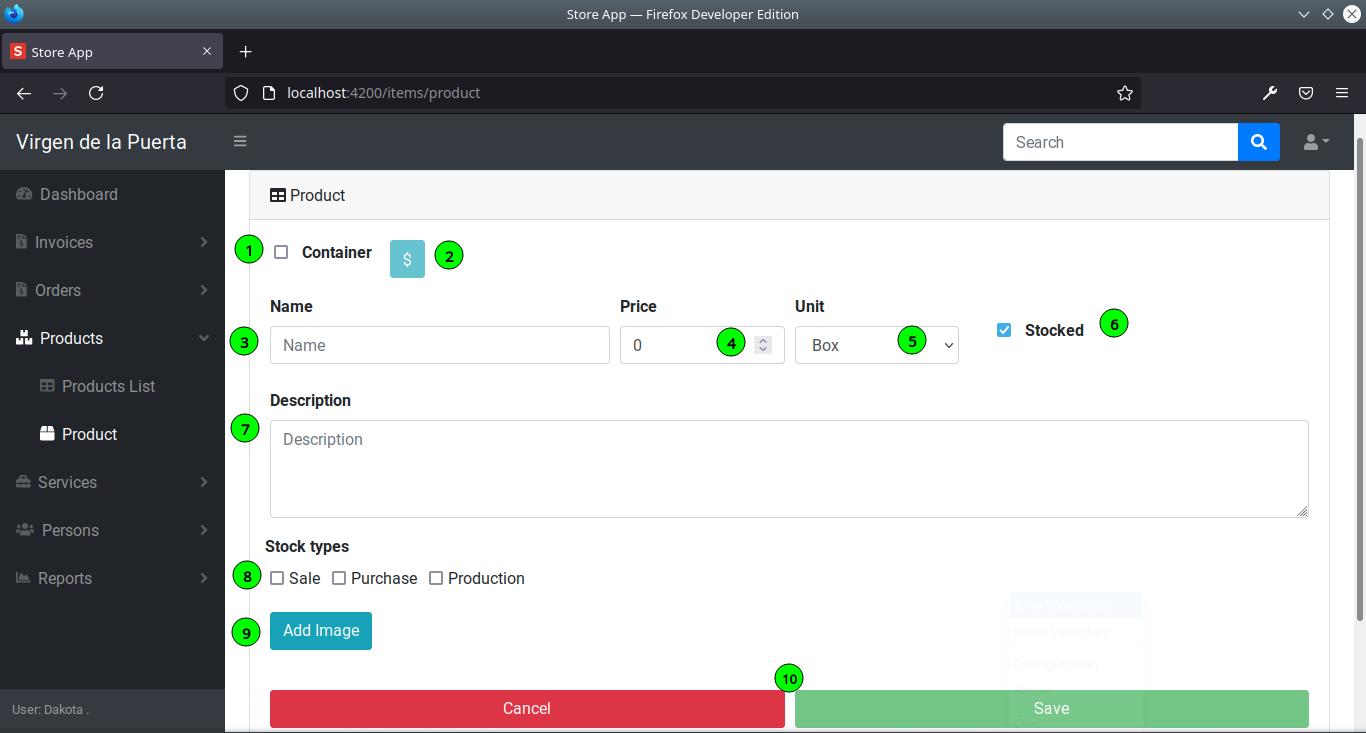
\includegraphics[width=\textwidth]{images/product_form-fields.png}
		\caption{product's fields}
		\label{fig:product_form-fields}
	\end{figure}
\end{enumerate}	

\subsubsection{Container's field}
\begin{enumerate}
	\item \textbf{Container}: it must be checked which means that a container will be created. A container has an amount of products.
	\item \textbf{Historic pricing}: show sell and purchase's price through time. If its only activate when a product is updated. See (Section~\ref{section:historic_pricing}).
	\item \textbf{Product's name}: search for the product that will belong to the container.
	\item \textbf{Amount}: amount of units of a container.
		\medskip
		\begin{leftbar}
			only available when container is checked.
		\end{leftbar}
	\item \textbf{Price}:  container's price.
		\medskip
		\begin{leftbar}
			\textbf{OPTIONAL FIELD}, can be fulfill later.
		\end{leftbar}
	\item \textbf{Unit}: it can be chosen between only options for container: \emph{box, package and back}
	\item \textbf{Stocked}: check if the container will have stock; otherwise, uncheck it.
	\item \textbf{Description}: container's description.
	\medskip
		\begin{leftbar}
			\textbf{OPTIONAL FIELD}
		\end{leftbar}
	\item \textbf{Stock types}: there are 3 types and they can be selected more than one.
		\begin{enumerate}
			\item \textbf{Sale}: if the product is going to be only sell, but not buy itself.
			\item \textbf{Purchase}: if the product is only bought but not sell.
			\item \textbf{Production}:  \InConstruction{}
		\end{enumerate}
	
	\item \textbf{Add image}: add product's image. See in (Section~\ref{section:add_image}).
		\medskip
		\begin{leftbar}
			\textbf{OPTIONAL FIELD}.
		\end{leftbar}  
	\item Click in \keys{save} to confirm the process; otherwise, Click in \keys{cancel} to abort it.
		\medskip
		\begin{leftbar}
			The process will be finished and the user will redirected to \textbf{Product List} page in (Section~\ref{section:product_list}).
		\end{leftbar}
	\begin{figure}[H]\centering
	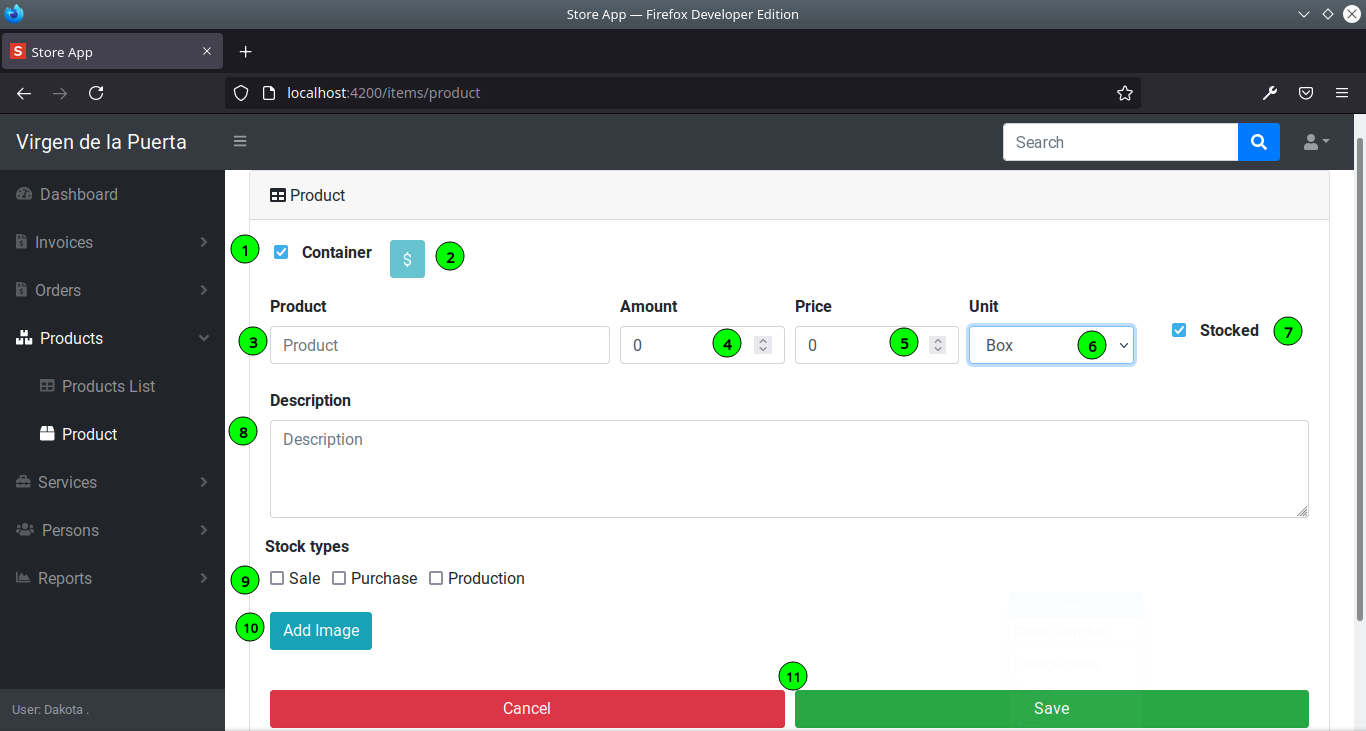
\includegraphics[width=\textwidth]{images/product_form-fields-container.png}
	\caption{container's fields}
	\label{fig:product_form-fields-container}
\end{figure}
\end{enumerate}	



\section{Service}
\subsection{Service List}\label{section:service_list}
\subsubsection{Access to module}
\begin{enumerate}
	\item From the left menu, click in  \menu{Services}
	\item From the left submenu, click in  \menu{Services List}
	\item The page will be showed.
	\medskip
	\begin{leftbar}
		Here there are some action that can be done with the items in the grid such as: \emph{search, edit, delete and print} .
	\end{leftbar}
	\begin{figure}[H]\centering
		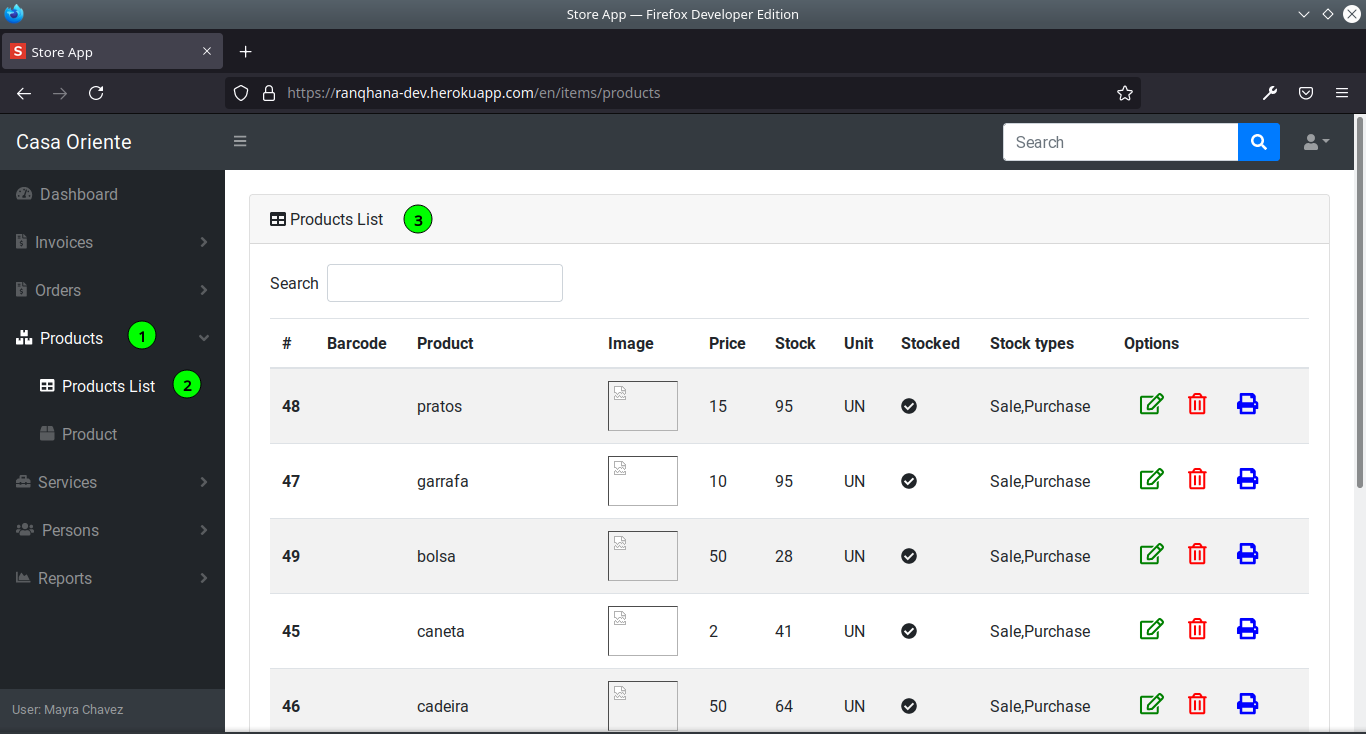
\includegraphics[width=\textwidth]{images/produc_list-access.png}
		\caption{access to module: Services List}
		\label{fig:service_list-access.png}
	\end{figure}
\end{enumerate}

\subsubsection{Search service}\label{section:service_search}
\begin{enumerate}
	\item Write the service name or part of that and it will be searched automatically.
	\begin{figure}[H]\centering
		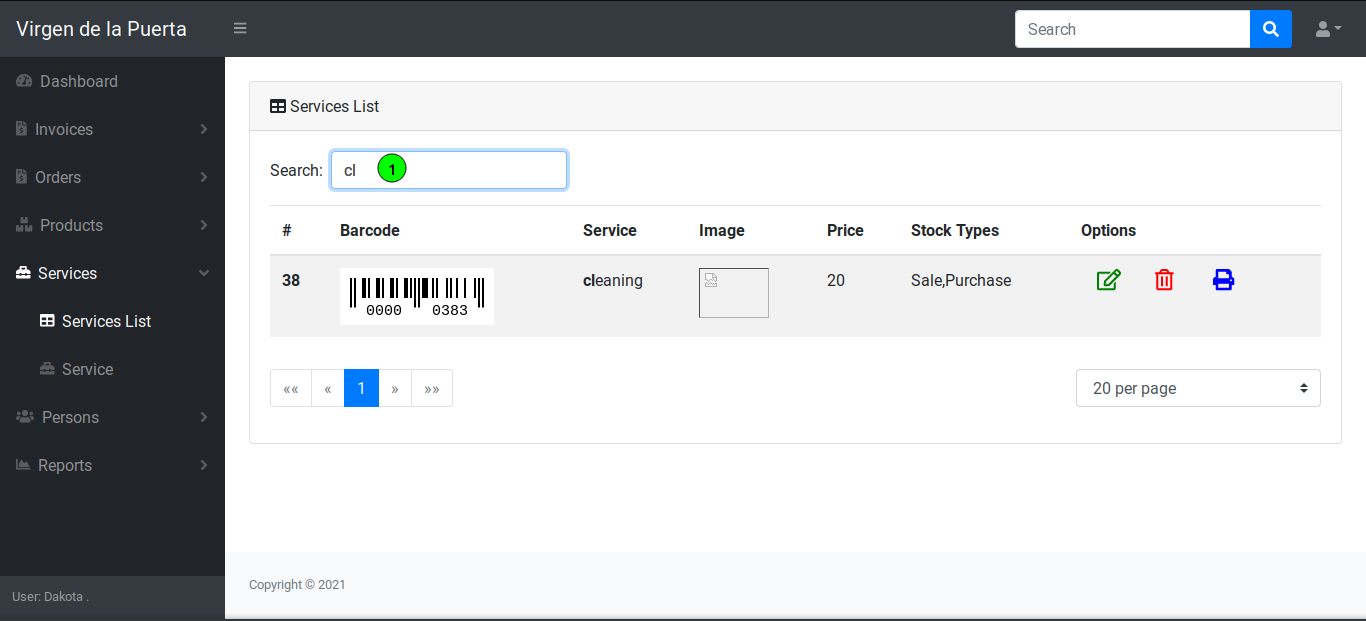
\includegraphics[width=\textwidth]{images/service_list-search.png}
		\caption{search service}
		\label{fig:service_list-search.png}
	\end{figure}
\end{enumerate}

\subsubsection{Delete service}
\begin{enumerate}
	\item Find the service to delete.
	\item Click in \faIcon{trash}.
	\begin{figure}[H]\centering
		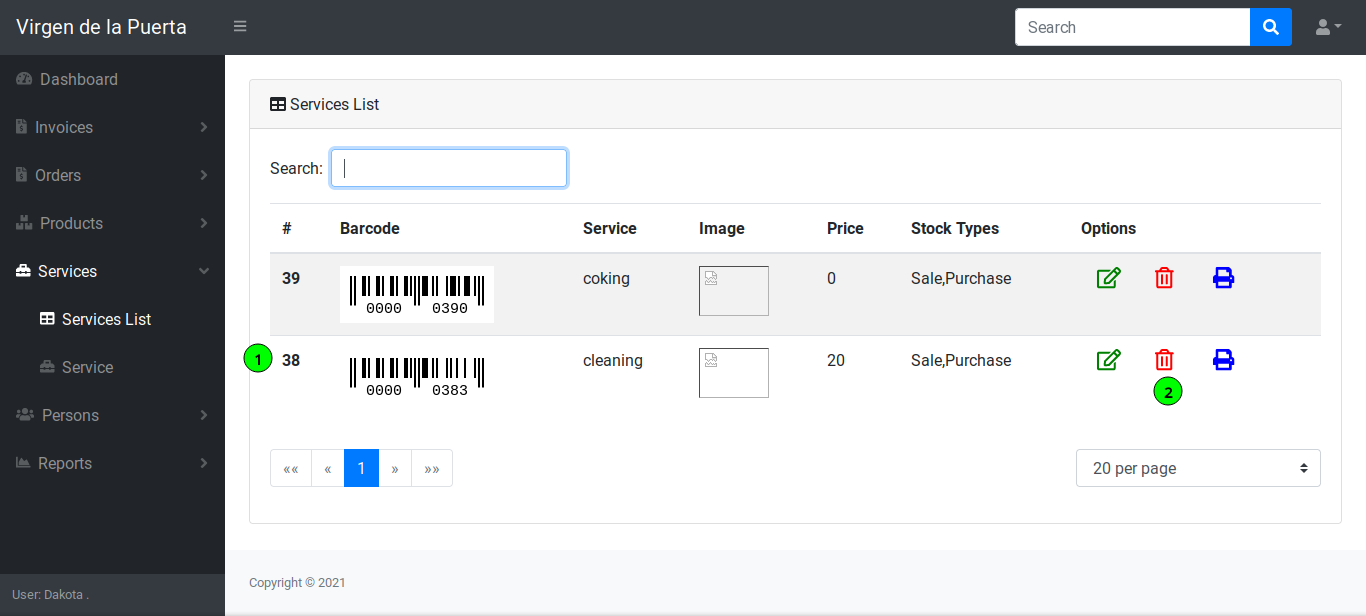
\includegraphics[width=\textwidth]{images/service_list-delete.png}
		\caption{delete service}
		\label{fig:service_list-delete.png}
	\end{figure}
	\item Click in \keys{yes} to confirm the delete; otherwise, Click in \keys{cancel} to abort the process.
	\begin{figure}[H]\centering
		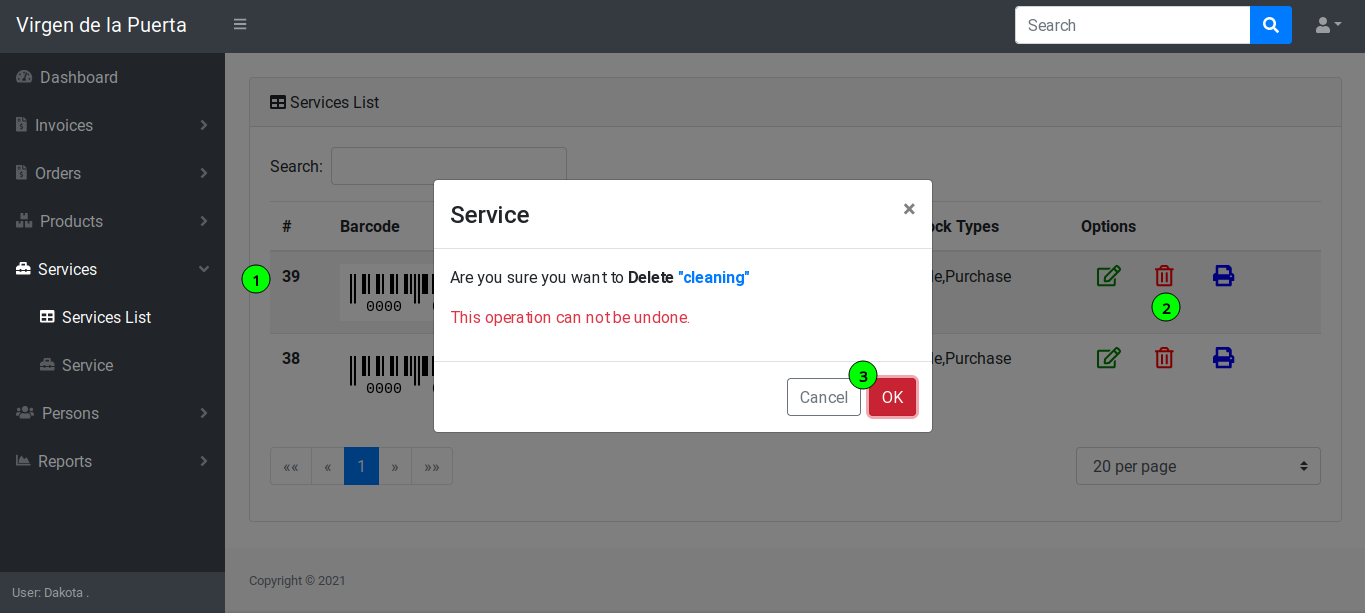
\includegraphics[width=\textwidth]{images/service_list-delete-modal.png}
		\caption{delete service: modal}
		\label{fig:service_list-delete-modal.png}
	\end{figure}
\end{enumerate}

\subsubsection{Update/Edit service}
\begin{enumerate}
	\item Find the service to edit.
	\item Click in \faIcon{edit}.
	\medskip
	\begin{leftbar}
		At that moment, it will be redirected to \textbf{Service Form} page.
	\end{leftbar}
	\begin{figure}[H]\centering
		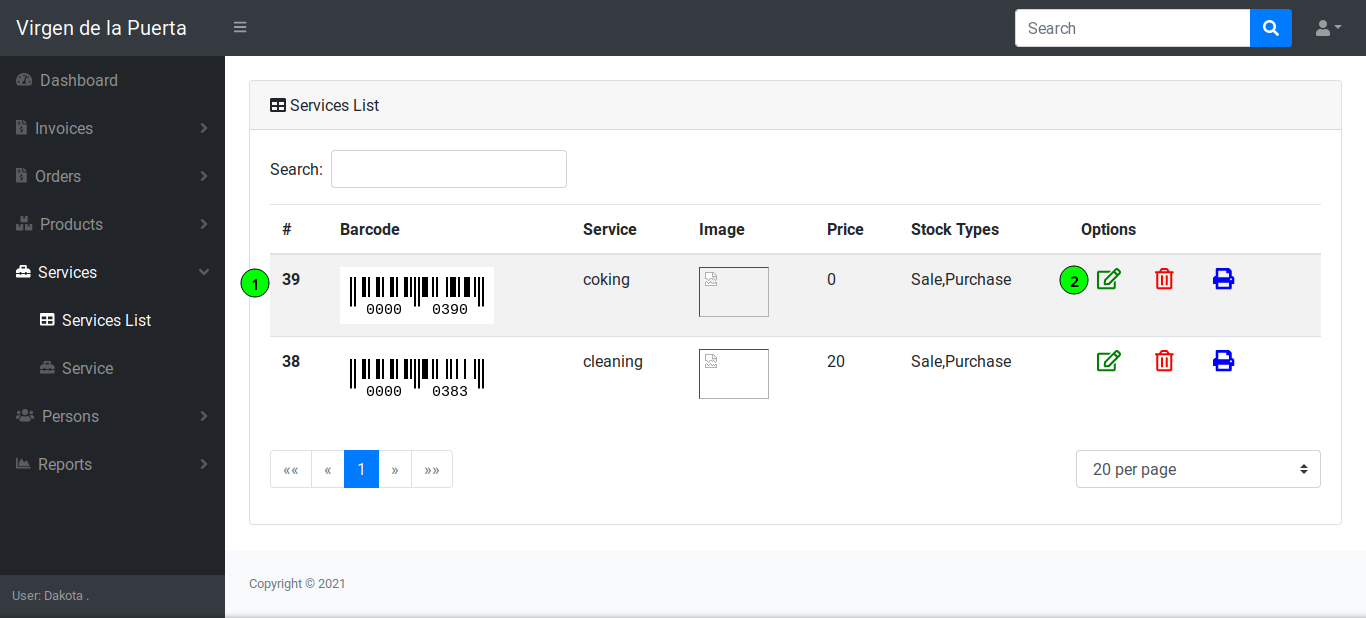
\includegraphics[width=\textwidth]{images/service_list-update.png}
		\caption{update/edit service}
		\label{fig:service_list-update.png}.
	\end{figure}
\end{enumerate}

\subsubsection{Print service}
\begin{enumerate}
	\item \InConstruction{}
\end{enumerate}

\subsection{Service Form}\label{section:service_form}
\subsubsection{Access to module}
\begin{enumerate}
	\item From the left menu, click in \menu{Services}
	\item From the left submenu, click in \menu{Service}
	\item The page will be showed.
	\medskip
	\begin{leftbar}
		Here 2 actions can be performed \emph{create and update} .
	\end{leftbar}
	\begin{figure}[H]\centering
		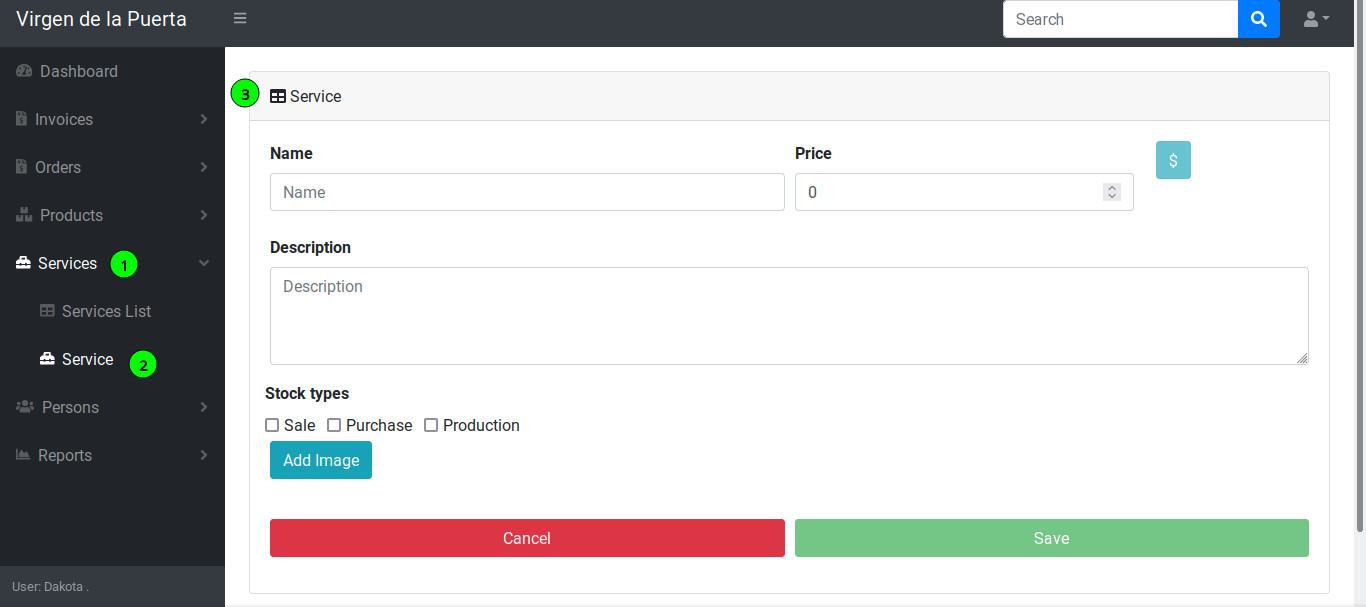
\includegraphics[width=\textwidth]{images/service_form-access.png}
		\caption{access to module: service}
		\label{fig:service_form-access.png}
	\end{figure}
\end{enumerate}

%%\subsection{Create Product}
\subsubsection{service's fields}
\begin{enumerate}
	\item \textbf{Name}: service's name.
	\item \textbf{Price}: service's price.
	\medskip
	\begin{leftbar}
		\textbf{OPTIONAL FIELD}, can be fulfill later.
	\end{leftbar}
	\item \textbf{Historic pricing}: show sell and purchase's price through time. If its only activate when a product is updated. See (Section~\ref{section:historic_pricing}).
	\item \textbf{Description}: product's description.
	\medskip
	\begin{leftbar}
		\textbf{OPTIONAL FIELD}
	\end{leftbar}
	\item \textbf{Stock types}: there are 3 types and they can be selected more than one.
		\begin{enumerate}
			\item \textbf{Sale}: if the product is going to be only sell, but not buy itself.
			\item \textbf{Purchase}: if the product is only bought but not sell.
			\item \textbf{Production}:  \InConstruction{}
		\end{enumerate}
	\item \textbf{Add image}: add product's image. See in (Section~\ref{section:add_image}).
	\medskip
	\begin{leftbar}
		\textbf{OPTIONAL FIELD}.
	\end{leftbar}
	\item Click in \keys{save} to confirm the process; otherwise, Click in \keys{cancel} to abort it.
		\medskip
		\begin{leftbar}
			The process will be finished and the user will redirected to \textbf{Product List} page.
		\end{leftbar}
	\begin{figure}[H]\centering
		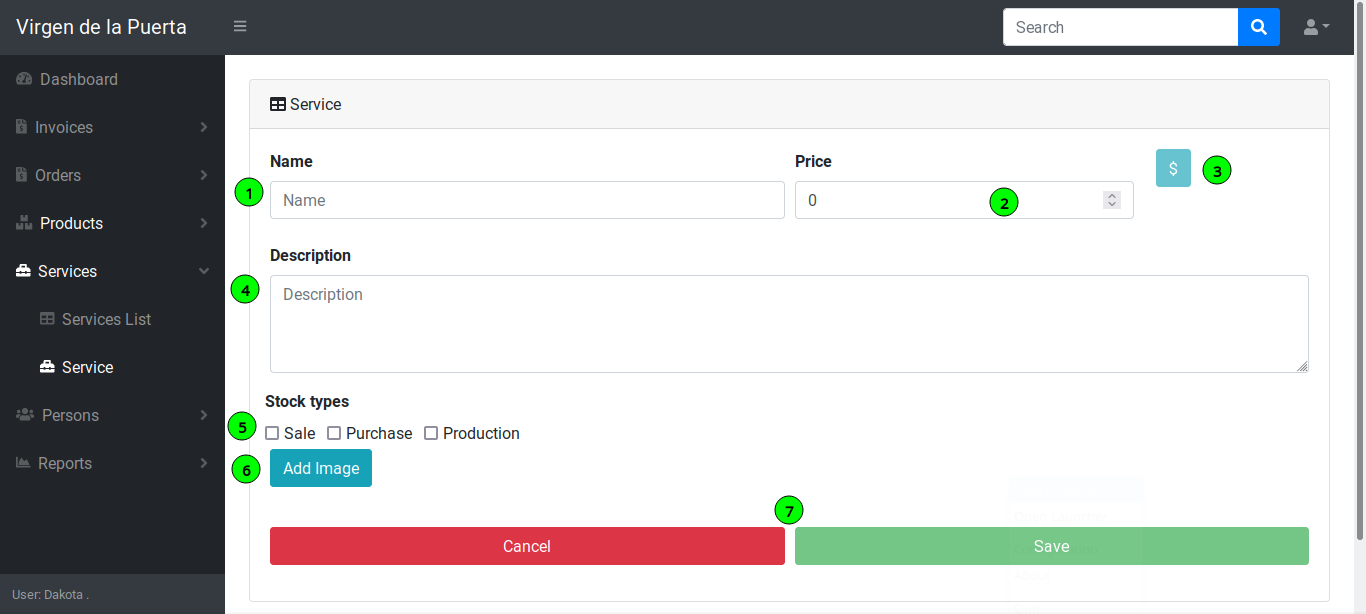
\includegraphics[width=\textwidth]{images/service_form-fields.png}
		\caption{service's fields}
		\label{fig:service_form-fields}
	\end{figure}
\end{enumerate}


\section{Persons}
\subsection{Users List}\label{section:user_list}
\subsubsection{Access to module}
\begin{enumerate}
	\item From the left menu, click in  \menu{Persons}
	\item From the left submenu, click in  \menu{My users list}
	\item The page will be showed.
	\medskip
	\begin{leftbar}
		Here there are some action that can be done with the items in the grid such as: \emph{search, edit and delete}.
	\end{leftbar}
	\begin{figure}[H]\centering
		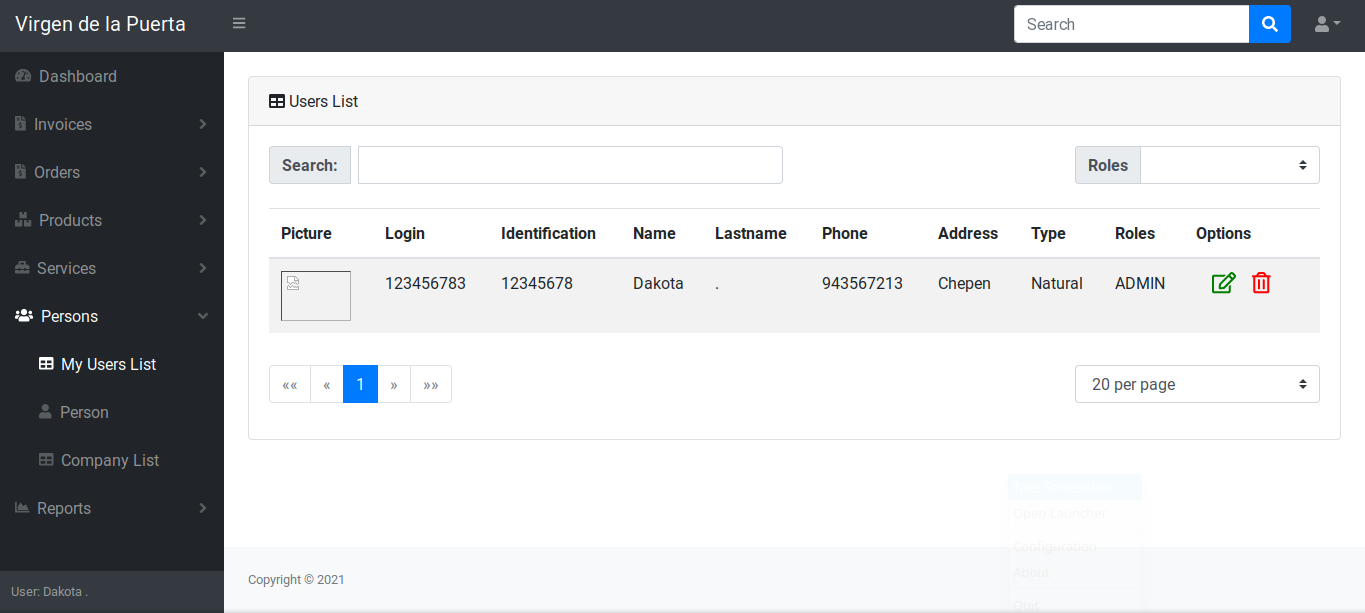
\includegraphics[width=\textwidth]{images/user_list-access.png}
		\caption{access to module: Services List}
		\label{fig:user_list-access}
	\end{figure}
\end{enumerate}

\subsubsection{Search user}\label{section:user_search}
\begin{enumerate}
	\item Write the user identification/name or part of that and it will be searched automatically.
	\item Select a role or in blank, which means search for all.
		\medskip
		\begin{leftbar}
			This option depends of your company and can be: \emph{user, admin and more} .
		\end{leftbar}
	\item Record(s) is showed.
	\begin{figure}[H]\centering
		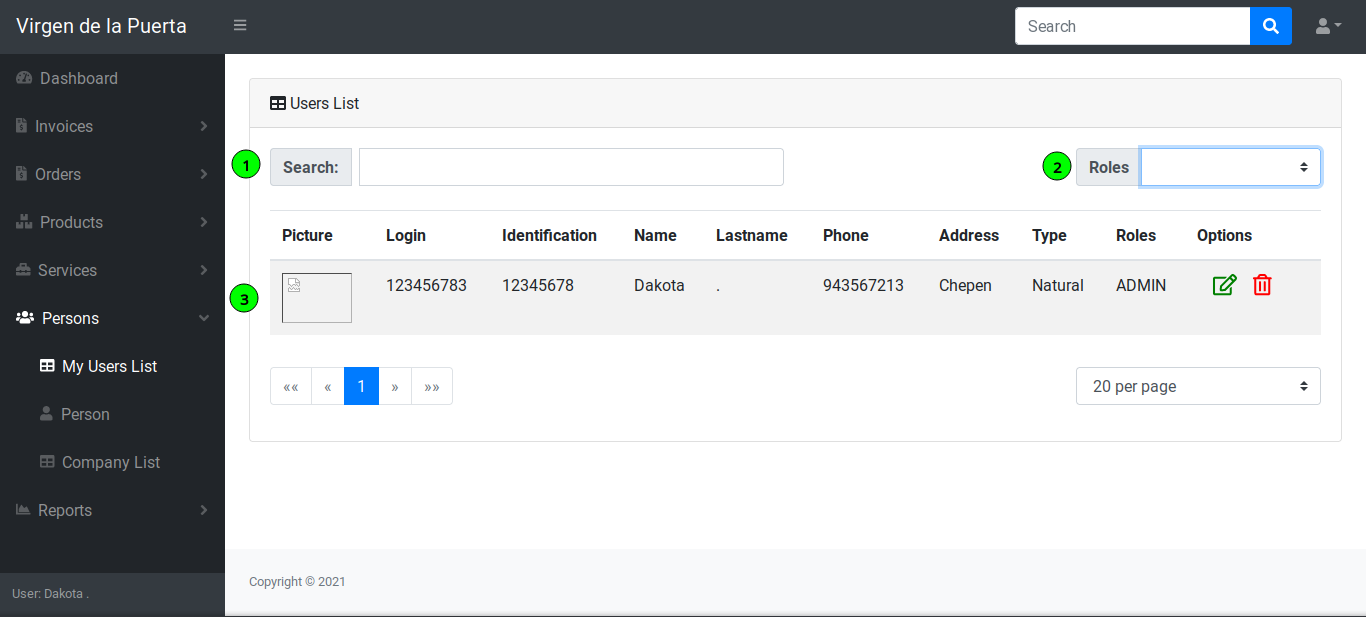
\includegraphics[width=\textwidth]{images/user_list-search.png}
		\caption{search user}
		\label{fig:user_list-search.png}
	\end{figure}
\end{enumerate}

\subsubsection{Delete user}
\begin{enumerate}
	\item Find the user to delete.
	\item Click in \faIcon{trash}.
	\begin{figure}[H]\centering
		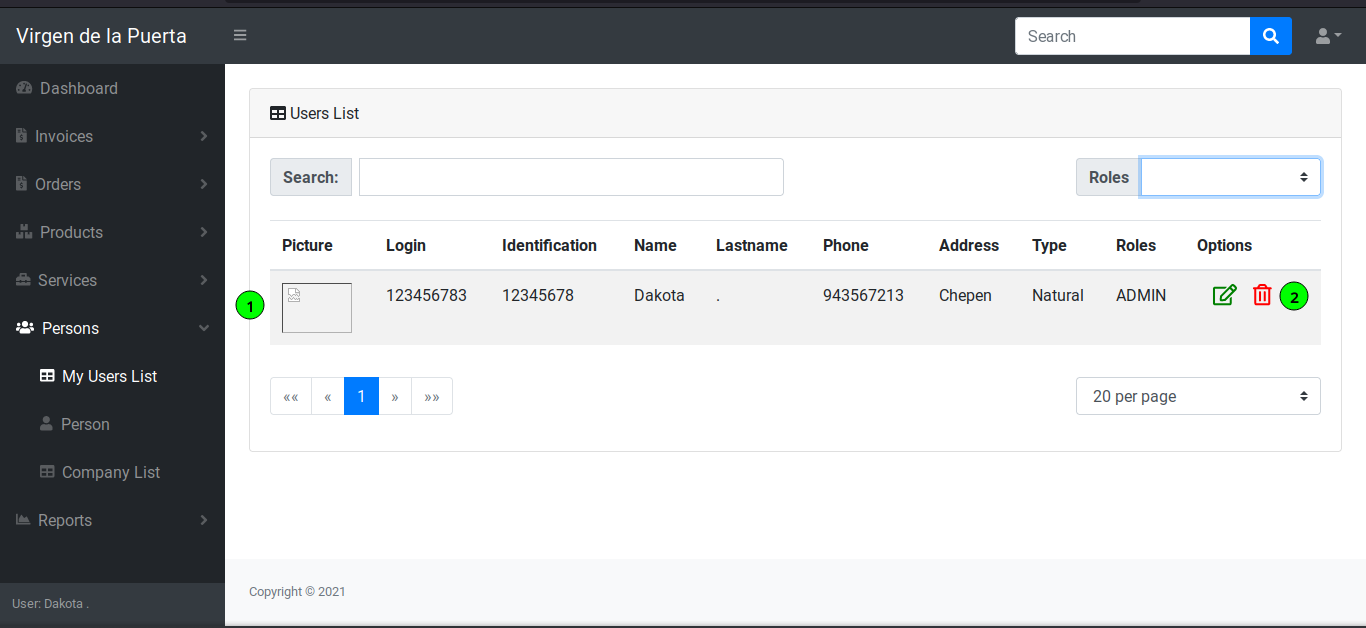
\includegraphics[width=\textwidth]{images/user_list-delete.png}
		\caption{delete user}
		\label{fig:user_list-delete.png}
	\end{figure}
	\item Click in \keys{yes} to confirm the delete; otherwise, Click in \keys{cancel} to abort the process.
	\begin{figure}[H]\centering
		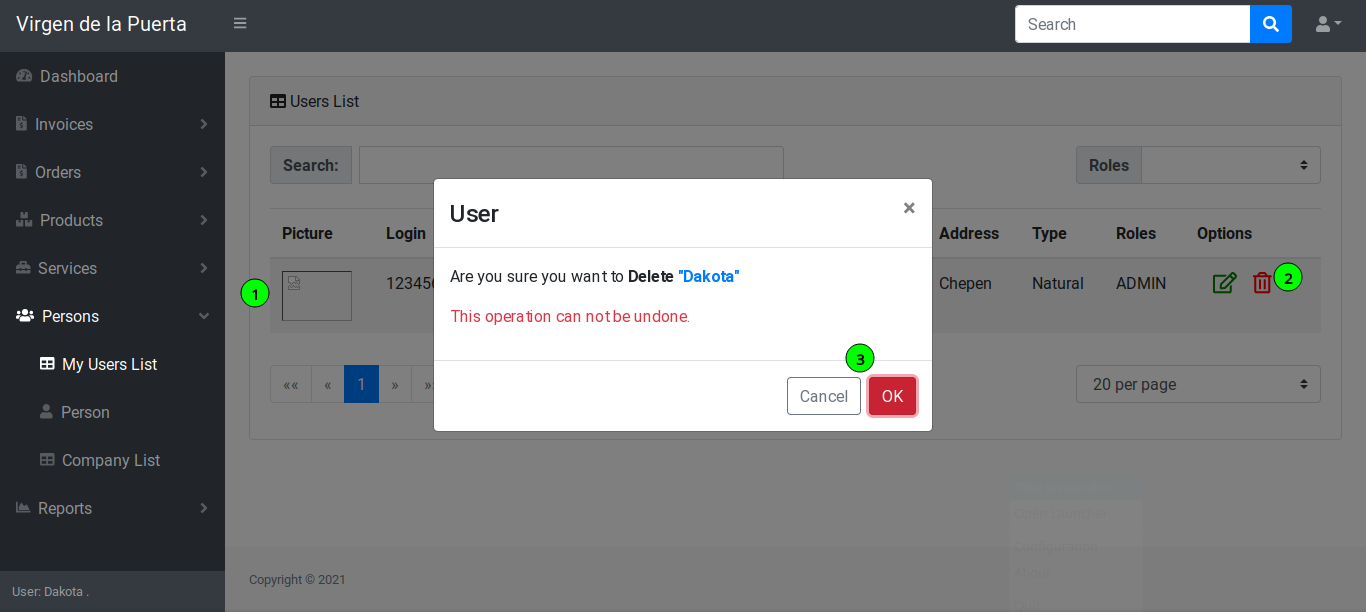
\includegraphics[width=\textwidth]{images/user_list-delete-modal.png}
		\caption{delete user: modal}
		\label{fig:user_list-delete-modal.png}
	\end{figure}
\end{enumerate}

\subsubsection{Update/Edit user}
\begin{enumerate}
	\item Find the user to edit.
	\item Click in \faIcon{edit}.
	\medskip
	\begin{leftbar}
		At that moment, it will be redirected to \textbf{Person Form} page in (Section~\ref{section:user_form}).
	\end{leftbar}
	\begin{figure}[H]\centering
		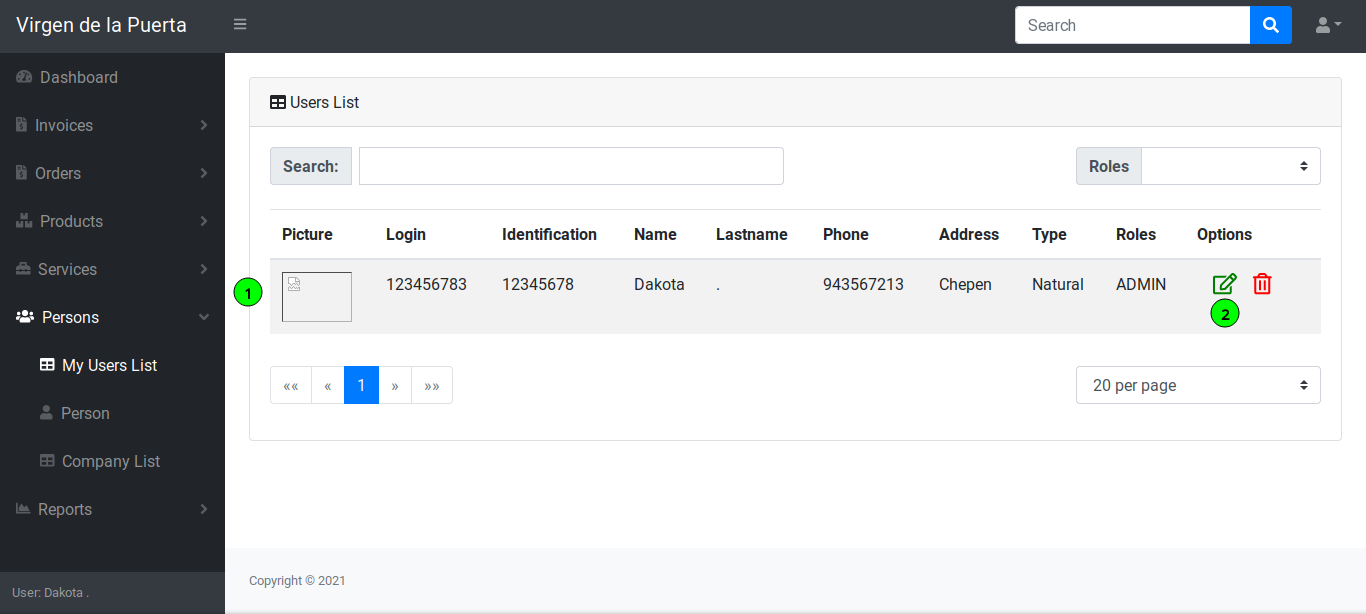
\includegraphics[width=\textwidth]{images/user_list-update.png}
		\caption{update/edit user}
		\label{fig:user_list-update.png}.
	\end{figure}
\end{enumerate}

\subsection{Person Form}\label{section:person_form}
\subsubsection{Access to module}
\begin{enumerate}
	\item From the left menu, click in \menu{Persons}
	\item From the left submenu, click in \menu{Person}
	\item The page will be showed.
	\medskip
	\begin{leftbar}
		Here 2 actions can be performed \emph{create and update} .
	\end{leftbar}
	\begin{figure}[H]\centering
		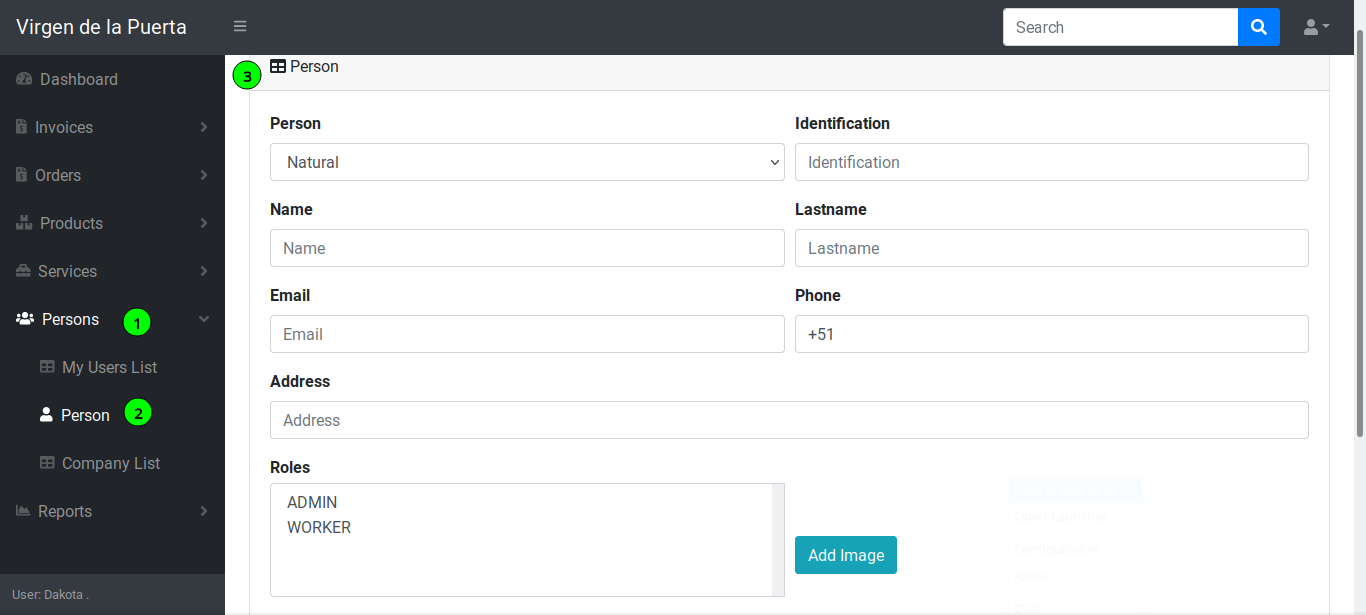
\includegraphics[width=\textwidth]{images/person_form-access.png}
		\caption{access to module: Person Form}
		\label{fig:person_form-access.png}
	\end{figure}
\end{enumerate}

\subsubsection{user's fields}\label{section:user_form}
\begin{enumerate}
	\item \textbf{Person}: to add an user, should be selected \textbf{Natural}.
	\item \textbf{Identification}: user's document identification number.
		\medskip
		\begin{leftbar}
			It is a numeric field and ask the ADMIN for which is going to be use here.
		\end{leftbar}
	\item \textbf{Name}: user's name.
	\item \textbf{lastname}: user's lastname.
	\item \textbf{E-mail}: user's e-mail.
	\item \textbf{Phone}: user's phone.
	\item \textbf{Address}: user's address.
		\medskip
		\begin{leftbar}
			\textbf{OPTIONAL FIELD}.
		\end{leftbar}
	\item \textbf{Roles}: roles of user in the application.
	\medskip
	\begin{leftbar}
		\textbf{OPTIONAL FIELD}, more than one can be selected and at least one is needed to user can access to the application.
	\end{leftbar}
	\item \textbf{Add image}: add product's image. See in (Section~\ref{section:add_image}).
	\medskip
	\begin{leftbar}
		\textbf{OPTIONAL FIELD}.
	\end{leftbar}
	\item Click in \keys{save} to confirm the process; otherwise, Click in \keys{cancel} to abort it.
	\medskip
	\begin{leftbar}
		The process will be finished and the user will redirected to \textbf{User List} page in (Section~\ref{section:user_list}).
	\end{leftbar}
	\begin{figure}[H]\centering
		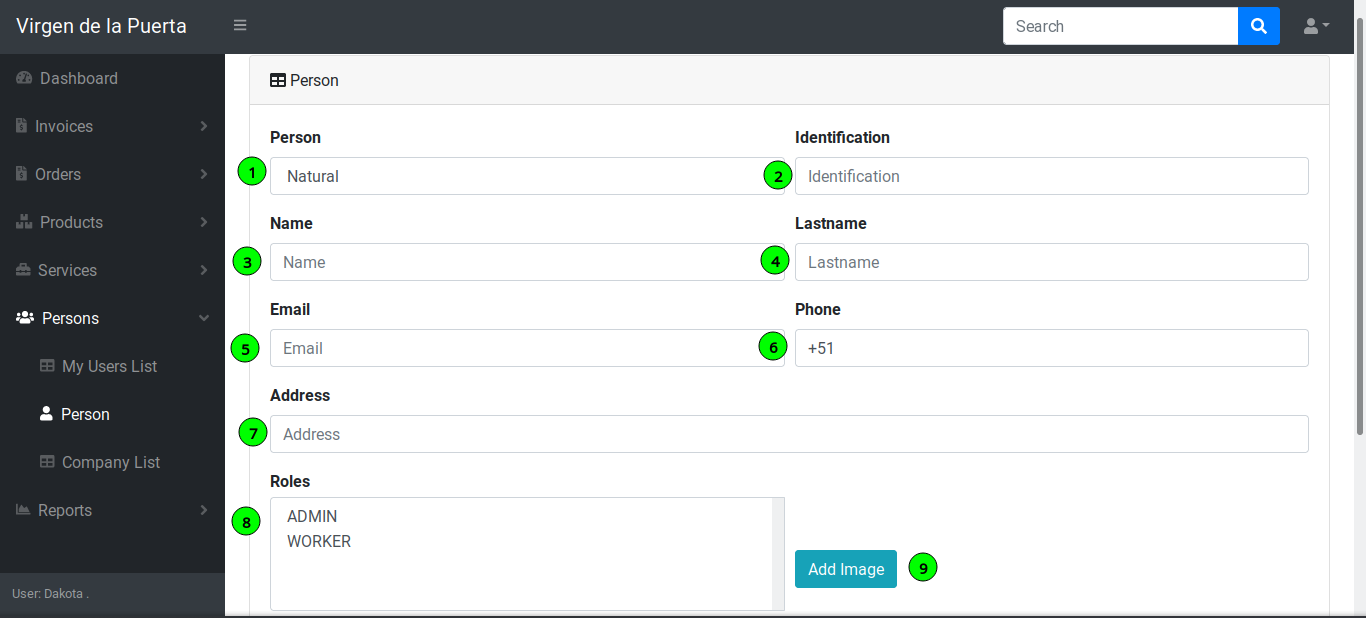
\includegraphics[width=\textwidth]{images/person_form-user-fields.png}
		\caption{user's fields}
		\label{fig:person_form-user-fields}
	\end{figure}
\end{enumerate}

\subsubsection{company's fields}\label{section:company_form}
\begin{enumerate}
	\item \textbf{Person}: to add a company, should be selected \textbf{Juridical}.
	\item \textbf{Identification}: company's document identification number.
	\medskip
	\begin{leftbar}
		It is a numeric field and ask the ADMIN for which is going to be use here.
	\end{leftbar}
	\item \textbf{Name}: company's name.
	\item \textbf{E-mail}: company's e-mail.
	\item \textbf{Phone}: company's phone.
	\item \textbf{Address}: company's address.
	\medskip
	\begin{leftbar}
		\textbf{OPTIONAL FIELD}.
	\end{leftbar}
	\item \textbf{Add image}: add product's image. See in (Section~\ref{section:add_image}).
	\medskip
	\begin{leftbar}
		\textbf{OPTIONAL FIELD}.
	\end{leftbar}
	\item Click in \keys{save} to confirm the process; otherwise, Click in \keys{cancel} to abort it.
	\medskip
	\begin{leftbar}
		The process will be finished and the user will redirected to \textbf{User List} page in (Section~\ref{section:user_list}).
	\end{leftbar}
	\begin{figure}[H]\centering
		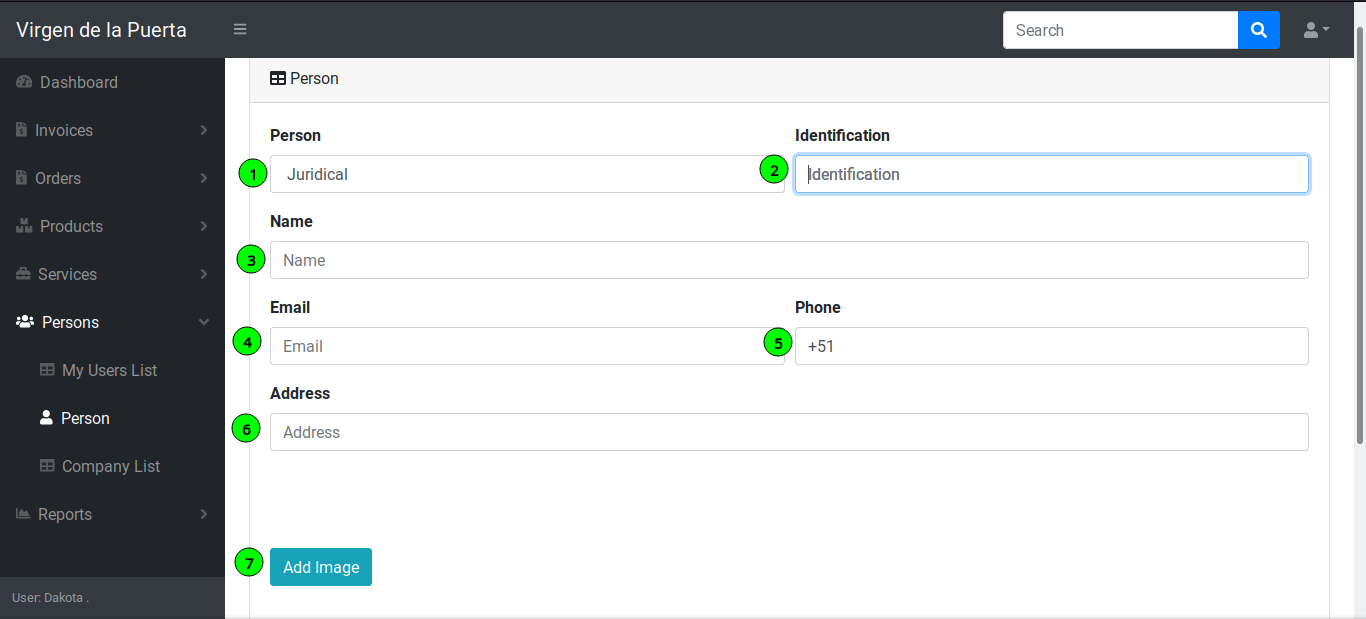
\includegraphics[width=\textwidth]{images/person_form-company-fields.png}
		\caption{company's fields}
		\label{fig:company_form-user-fields}
	\end{figure}
\end{enumerate}


\subsection{Companies List}\label{section:company_list}
\subsubsection{Access to module}
\begin{enumerate}
	\item From the left menu, click in  \menu{Persons}
	\item From the left submenu, click in  \menu{Company list}
	\item The page will be showed.
	\medskip
	\begin{leftbar}
		Here there are some action that can be done with the items in the grid such as: \emph{search, edit and delete}. The last 2 actions are allowed only for your companies.
	\end{leftbar}
	\begin{figure}[H]\centering
		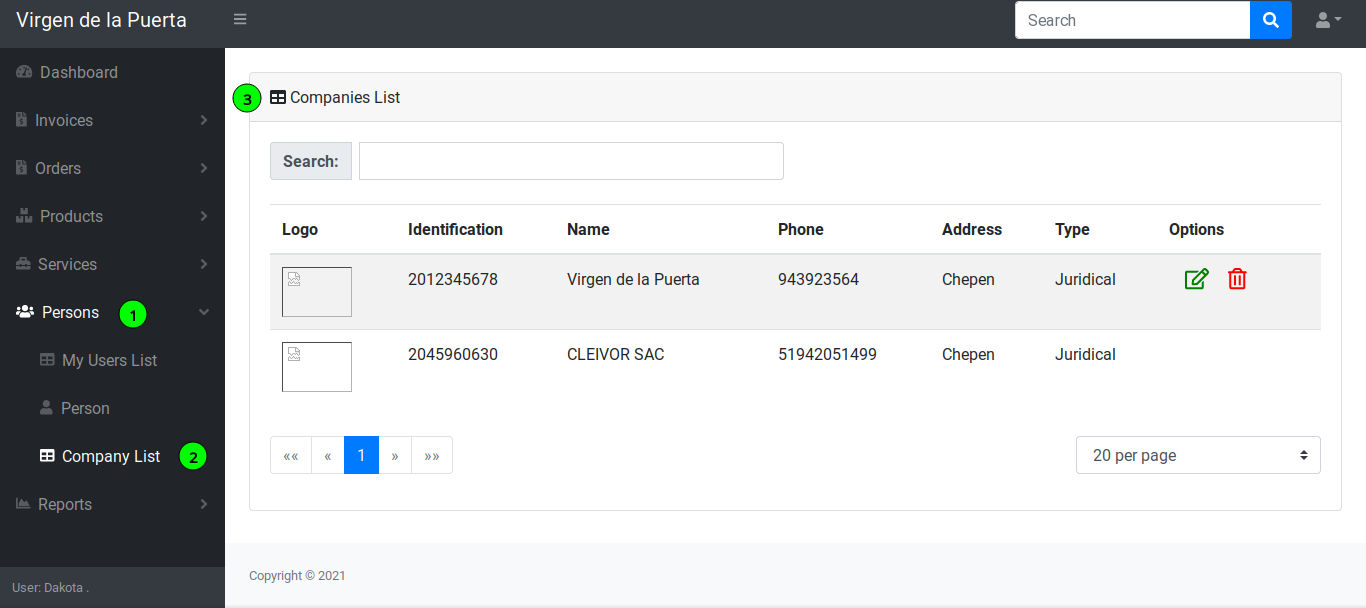
\includegraphics[width=\textwidth]{images/company_list-access.png}
		\caption{access to module: Companies List}
		\label{fig:company_list-access}
	\end{figure}
\end{enumerate}

\subsubsection{Search company}\label{section:company_search}
\begin{enumerate}
	\item Write the company identification/name or part of that and it will be searched automatically.
	\item Record(s) is showed.
	\begin{figure}[H]\centering
		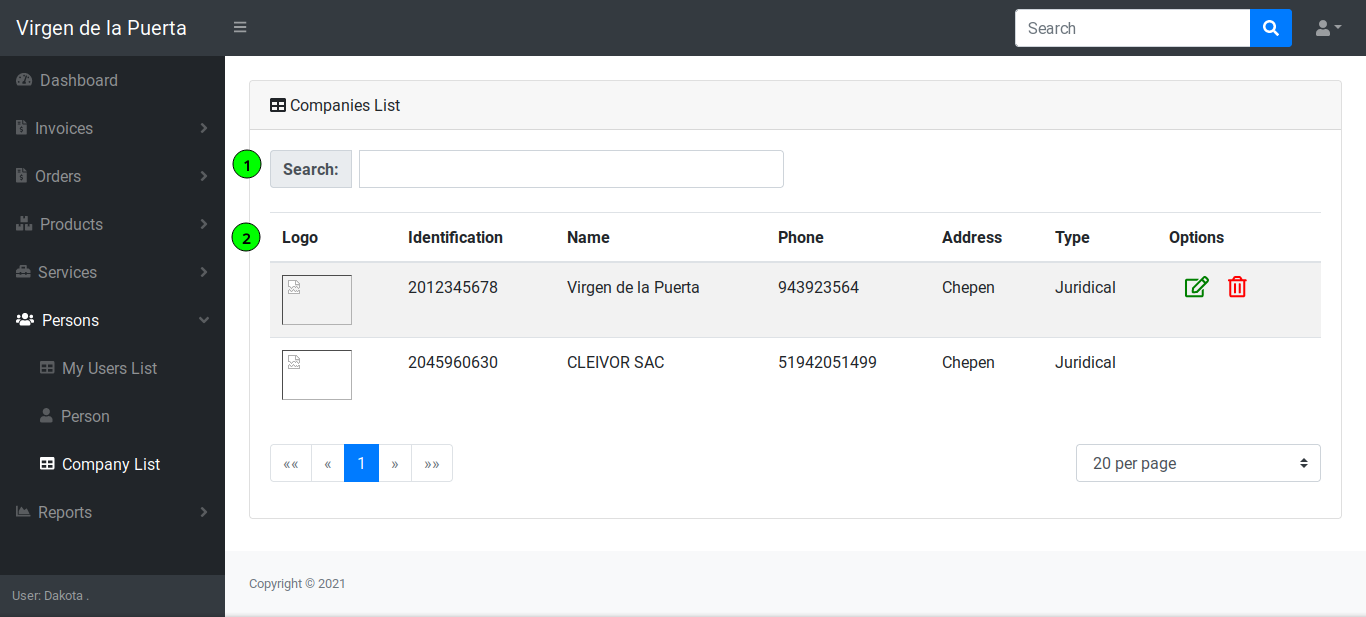
\includegraphics[width=\textwidth]{images/company_list-search.png}
		\caption{search company}
		\label{fig:company_list-search}
	\end{figure}
\end{enumerate}

\subsubsection{Delete company}
\begin{enumerate}
	\item Find the company to delete.
	\item Click in \faIcon{trash}.
	\begin{figure}[H]\centering
		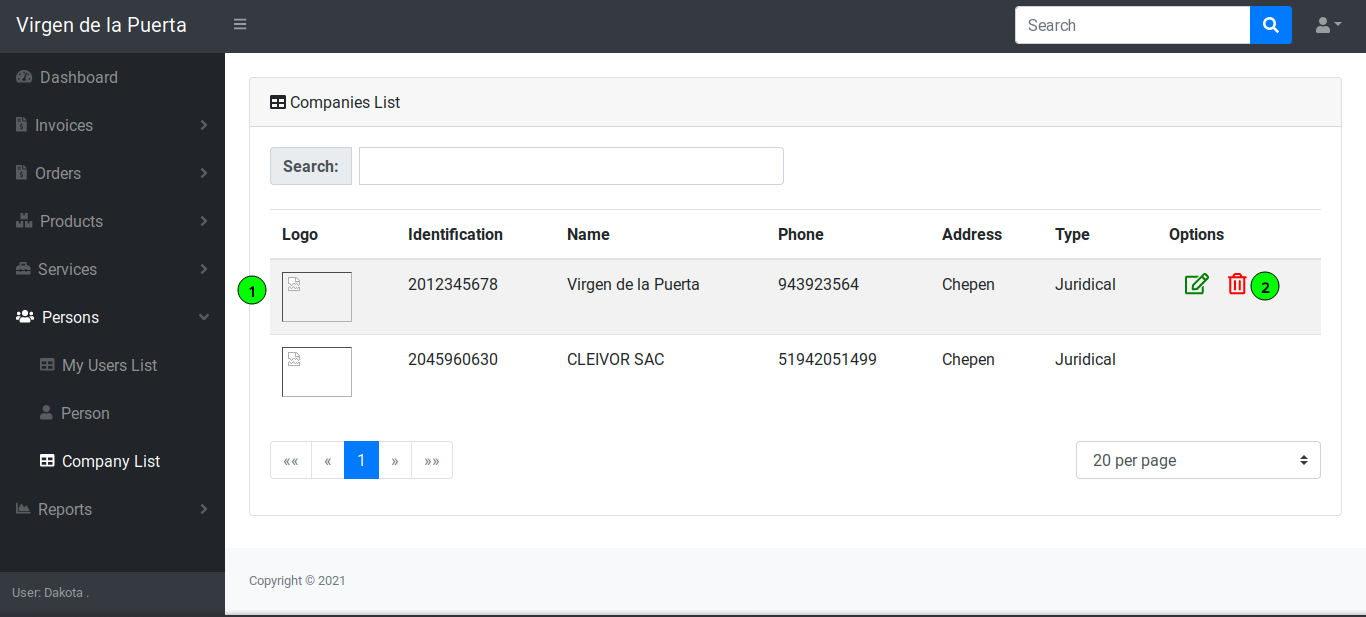
\includegraphics[width=\textwidth]{images/company_list-delete.png}
		\caption{delete company}
		\label{fig:company_list-delete}
	\end{figure}
	\item Click in \keys{yes} to confirm the delete; otherwise, Click in \keys{cancel} to abort the process.
	\begin{figure}[H]\centering
		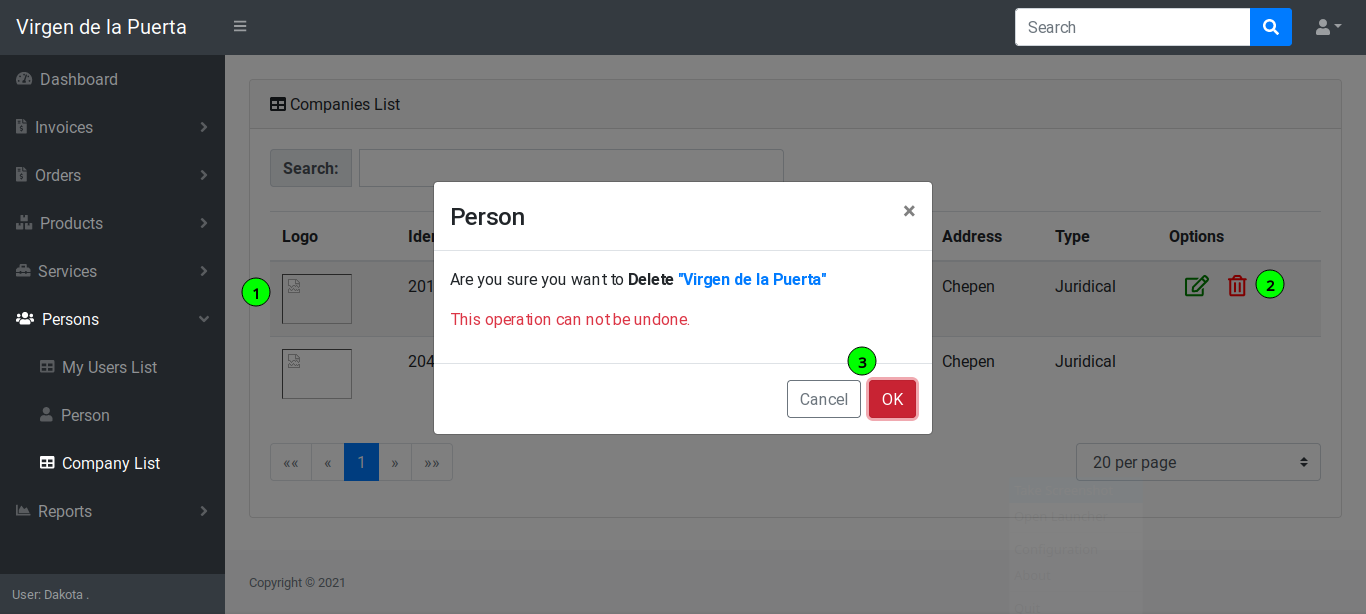
\includegraphics[width=\textwidth]{images/company_list-delete-modal.png}
		\caption{delete company: modal}
		\label{fig:company_list-delete-modal}
	\end{figure}
\end{enumerate}

\subsubsection{Update/Edit company}
\begin{enumerate}
	\item Find the company to edit.
	\item Click in \faIcon{edit}.
	\medskip
	\begin{leftbar}
		At that moment, it will be redirected to \textbf{Company Form} page in (Section~\ref{section:company_form}).
	\end{leftbar}
	\begin{figure}[H]\centering
		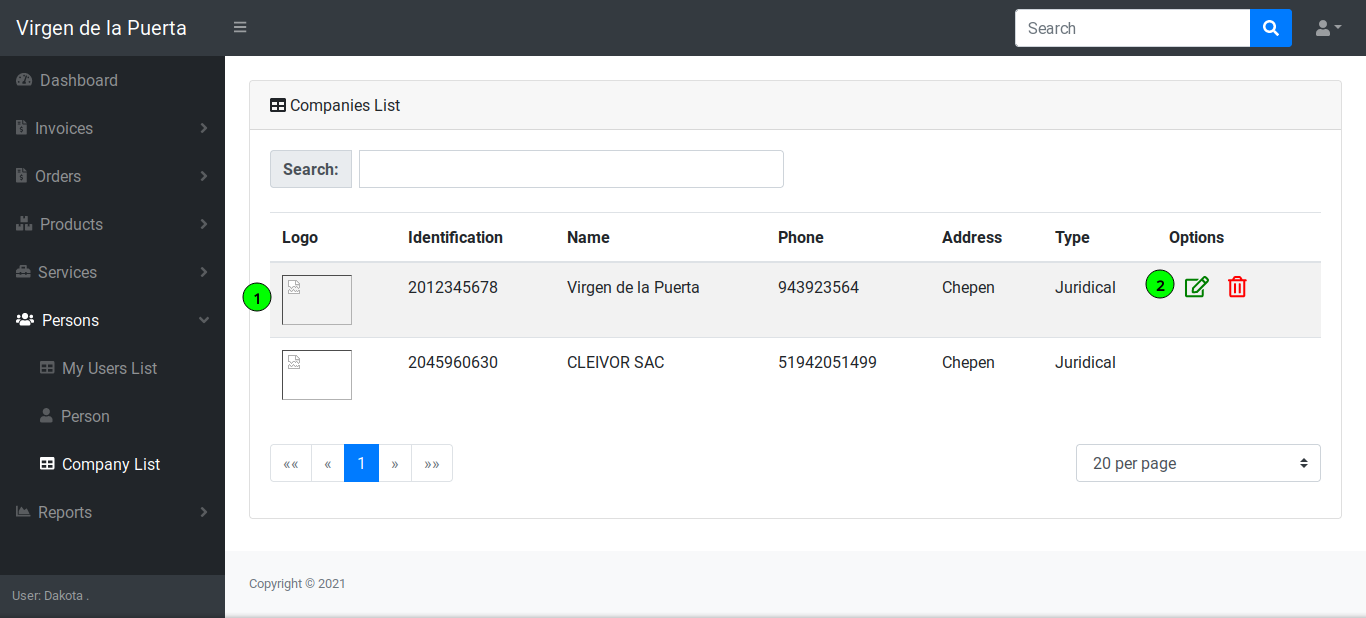
\includegraphics[width=\textwidth]{images/company_list-update.png}
		\caption{update/edit company}
		\label{fig:company_list-update}.
	\end{figure}
\end{enumerate}

\section{Reports}
\subsection{Invoice money by payment type}\label{section:invoice_money_by_payment_type}
\subsubsection{Access to module}
\begin{enumerate}
	\item From the left menu, click in  \menu{Reports}
	\item From the left submenu, click in \menu{Invoice \$\$\$ by payment type}
	\item The page will be showed.
	\begin{figure}[H]\centering
		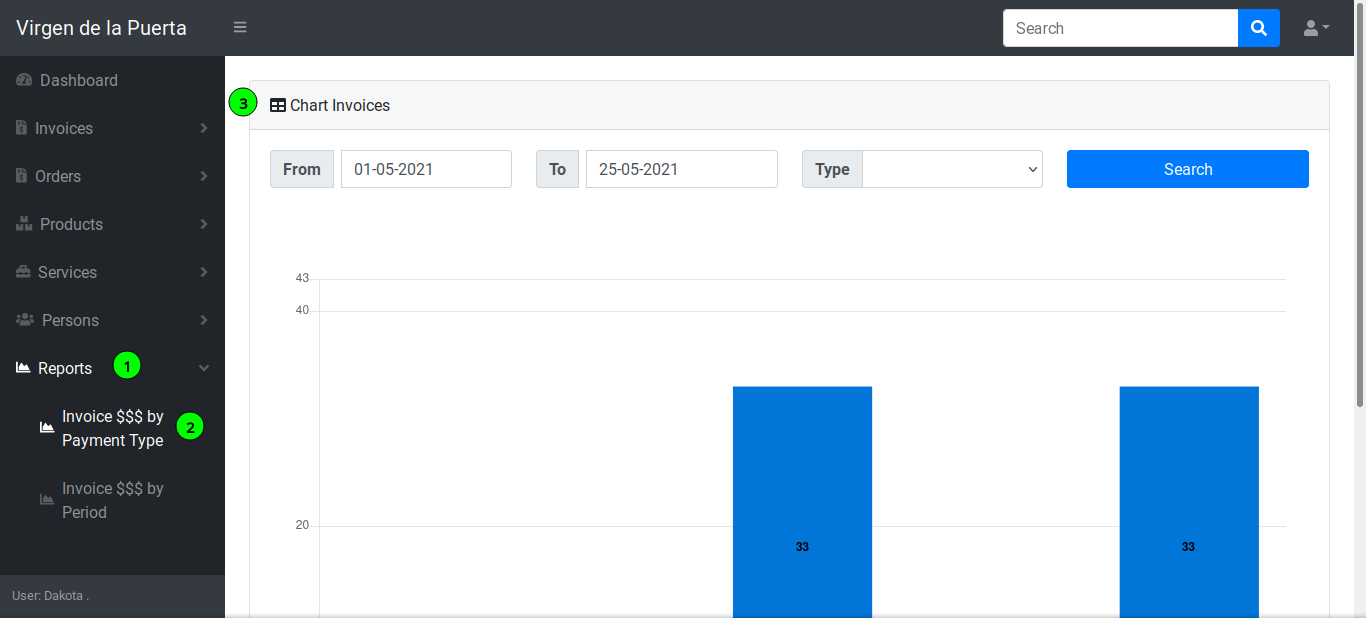
\includegraphics[width=\textwidth]{images/report_invoice_by_payment_type-access.png}
		\caption{access to module: Invoice money by payment type}
		\label{fig:report_invoice_by_payment_type-access}
	\end{figure}
\end{enumerate}

\subsubsection{Search}\label{section:invoice_money_by_payment_type_search}
\begin{enumerate}
	\item \textbf{From}: initial date in search range.
	\item \textbf{To}: final date in search range.
	\item \textbf{Type}: it is the type of invoice and it can selected one option or in blank, which means will search for all.
		\medskip
		\begin{leftbar}
			Options: \emph{sell or purchase} .
		\end{leftbar}
	\item Click in \keys{search}
	\begin{figure}[H]\centering
		\includegraphics[width=\textwidth]{images/report_invoice_by_payment_type-search.png}
		\caption{search}
		\label{fig:report_invoice_by_payment_type-search}
	\end{figure}
	\item Result graph is showed in (Section~\ref{section:invoice_money_by_payment_type_result}).
\end{enumerate}

\subsubsection{Result}\label{section:invoice_money_by_payment_type_result}
Each column represents amount of money depends on search's parameters.
\begin{enumerate}
	\item \textbf{Debit}: transactions paid using debit card.
	\item \textbf{Credit}: transactions paid using credit card.
	\item \textbf{Cash}: transactions paid with cash.
	\item \textbf{Store credit}: transactions offers with internal credit from the store.
	\item \textbf{Total}: sum of the last transactions' values.
	\begin{figure}[H]\centering
		\includegraphics[width=\textwidth]{images/report_invoice_by_payment_type-result1.png}
		\caption{result}
		\label{fig:report_invoice_by_payment_type-result1}
	\end{figure}
\end{enumerate}

\subsection{Invoice money by period}\label{section:invoice_money_by_period}
\subsubsection{Access to module}
\begin{enumerate}
	\item From the left menu, click in  \menu{Reports}
	\item From the left submenu, click in \menu{Invoice \$\$\$ by period}
	\item The page will be showed.
	\begin{figure}[H]\centering
		\includegraphics[width=\textwidth]{images/report_invoice_by_period-access.png}
		\caption{access to module: Invoice money by period}
		\label{fig:report_invoice_by_period-access}
	\end{figure}
\end{enumerate}

\subsubsection{Search \& Result}\label{section:invoice_money_by_period_search}
\begin{enumerate}
	\item \textbf{From}: initial date in search range.
	\item \textbf{To}: final date in search range.
	\item \textbf{Type}: it is the type of invoice and it can selected one option or in blank, which means will search for all.
	\medskip
	\begin{leftbar}
		Options: \emph{sell or purchase}.
	\end{leftbar}
	\item \textbf{By}: it is the period by what it will be searched.
	\medskip
	\begin{leftbar}
		Options: \emph{hour, day, month and year}.
	\end{leftbar}
	\item Click in \keys{search}
	\begin{figure}[H]\centering
		\includegraphics[width=\textwidth]{images/report_invoice_by_period-search.png}
		\caption{search}
		\label{fig:report_invoice_by_period-search}
	\end{figure}
	\item Result graph is showed.
	\begin{figure}[H]\centering
		\includegraphics[width=\textwidth]{images/report_invoice_by_period-result.png}
		\caption{result}
		\label{fig:report_invoice_by_period-result1}
	\end{figure}
\end{enumerate}

\section{Others modules}
\subsection{Images}
\subsubsection{Add image}\label{section:add_image}
\begin{enumerate}
	\item Click in \keys{add images}
	\medskip
	\begin{leftbar}
		This button is showed in many modules such as: \emph{products, services and users}
	\end{leftbar}
	\begin{figure}[H]\centering
		\includegraphics[width=\textwidth]{images/image-clickIn.png}
		\caption{image click in}
		\label{fig:image-clickIn}
	\end{figure}
	\item Click in \keys{choose image}
	\begin{figure}[H]\centering
		\includegraphics[width=\textwidth]{images/image-modal.png}
		\caption{image modal}
		\label{fig:image-modal}
	\end{figure}
	\item A window will be opened to browser the image in the computer.
	\item Select the image
	\item Click in \keys{open} to confirm the selection; otherwise, click in \keys{cancel} to abort the process.
	\begin{figure}[H]\centering
		\includegraphics[width=\textwidth]{images/image-choose.png}
		\caption{image choose}
		\label{fig:image-choose}
	\end{figure}
	\item Click in \keys{ok} to save the image; otherwise, click in \keys{cancel} to abort the process.
	\begin{figure}[H]\centering
		\includegraphics[width=\textwidth]{images/image-save.png}
		\caption{image save}
		\label{fig:image-save}
	\end{figure}
	\item Finally, the image will be showed .
	\begin{figure}[H]\centering
		\includegraphics[width=\textwidth]{images/image-show.png}
		\caption{image show}
		\label{fig:image-show}
	\end{figure}
\end{enumerate}

\subsubsection{Delete image}
\begin{enumerate}
	\item Find the image to delete.
	\item Click in \faIcon{trash}.
	\begin{figure}[H]\centering
		\includegraphics[width=\textwidth]{images/image-delete.png}
		\caption{delete image}
		\label{fig:image-delete.png}
	\end{figure}
	\item Click in \keys{yes} to confirm the delete; otherwise, click in \keys{cancel} to abort the process.
	\begin{figure}[H]\centering
		\includegraphics[width=\textwidth]{images/image-delete-modal.png}
		\caption{delete image: modal}
		\label{fig:image-delete-modal.png}
	\end{figure}
\end{enumerate}

\subsection{Made Payment}\label{section:made_payment}
\begin{enumerate}
	\item Write the amount of cash.
	\item If there is an exchange, it will be showed.
	\item Click in \keys{Pay}
	\medskip
	\begin{leftbar}
		the process will be finished and the user will redirected to \textbf{Invoice List} page in (Section~\ref{section:invoice_list}).
	\end{leftbar}
	\begin{figure}[H]\centering
		\includegraphics[width=\textwidth]{images/sellinvoice-7}
		\caption{made payment}\label{fig:sellinvoice-7}
	\end{figure}
\end{enumerate}

\subsection{Historic Pricing}\label{section:historic_pricing}
\begin{enumerate}
	\item Find the item.
	\medskip
	\begin{leftbar}
		Item can be a product (Section~\ref{section:product_search}) or a service (Section~\ref{section:service_search})
	\end{leftbar}
	\item Click in \faIcon{edit}.
	\medskip
	\begin{leftbar}
		At that moment, it will be redirected to \textbf{Product Form} page in (Section~\ref{section:product_form}) or to \textbf{Service Form} page in (Section~\ref{section:service_form}).
	\end{leftbar}
	\begin{figure}[H]\centering
		\includegraphics[width=\textwidth]{images/produc_list-update.png}
		\caption{select product}
		\label{fig:select-product.png}.
	\end{figure}
	\item Click in \keys{\$}.
	\begin{figure}[H]\centering
		\includegraphics[width=\textwidth]{images/historing_price-open.png}
		\caption{historing price: open}
		\label{fig:historing_price-open}
	\end{figure}
	\item A modal will show sell and purchase's prices.
	\item Click in \keys{close} to exit.
	\begin{figure}[H]\centering
		\includegraphics[width=\textwidth]{images/historing_price-modal.png}
		\caption{historing price}
		\label{fig:historing_price-modal}
	\end{figure}
	
\end{enumerate}	

\subsection{Change language}\label{section:change_language}
\subsubsection{Access to module from Login}
This option is found in \textbf{Login} page. (Section~\ref{section:login_app}).
\begin{enumerate}
	\item Click in link \textbf{\emph{Change language}}
	\begin{figure}[H]\centering
		\includegraphics[width=\textwidth]{images/change_language-login.png}
		\caption{access to module from login}
		\label{fig:change_language-login}
	\end{figure}
\end{enumerate}

\subsubsection{Access to module from System}
This option is found from up panel at any page in the system.
\begin{enumerate}
	\item Click in icon \faIcon{user}
	\item Click in option \textbf{\emph{Change language}}
	\begin{figure}[H]\centering
		\includegraphics[width=\textwidth]{images/change_language-system.png}
		\caption{access to module from system}
		\label{fig:change_language-system}
	\end{figure}
\end{enumerate}

\subsubsection{Change}
\begin{enumerate}
	\item Select language.
		\medskip
		\begin{leftbar}
			options: \emph{English, Spanish and Portuguese}.
		\end{leftbar}
	\item Click in \keys{yes} to confirm the change; otherwise, Click in \keys{cancel} to abort the process.
	\begin{figure}[H]\centering
		\includegraphics[width=\textwidth]{images/change_language-modal.png}
		\caption{change language: modal}
		\label{change_language-modal}
	\end{figure}
\end{enumerate}



\bibliographystyle{plain}
\bibliography{refs}
\end{document}